\documentclass[11pt]{article}

    \usepackage[breakable]{tcolorbox}
    \usepackage{parskip} % Stop auto-indenting (to mimic markdown behaviour)
    

    % Basic figure setup, for now with no caption control since it's done
    % automatically by Pandoc (which extracts ![](path) syntax from Markdown).
    \usepackage{graphicx}
    % Maintain compatibility with old templates. Remove in nbconvert 6.0
    \let\Oldincludegraphics\includegraphics
    % Ensure that by default, figures have no caption (until we provide a
    % proper Figure object with a Caption API and a way to capture that
    % in the conversion process - todo).
    \usepackage{caption}
    \DeclareCaptionFormat{nocaption}{}
    \captionsetup{format=nocaption,aboveskip=0pt,belowskip=0pt}

    \usepackage{float}
    \floatplacement{figure}{H} % forces figures to be placed at the correct location
    \usepackage{xcolor} % Allow colors to be defined
    \usepackage{enumerate} % Needed for markdown enumerations to work
    \usepackage{geometry} % Used to adjust the document margins
    \usepackage{amsmath} % Equations
    \usepackage{amssymb} % Equations
    \usepackage{textcomp} % defines textquotesingle
    % Hack from http://tex.stackexchange.com/a/47451/13684:
    \AtBeginDocument{%
        \def\PYZsq{\textquotesingle}% Upright quotes in Pygmentized code
    }
    \usepackage{upquote} % Upright quotes for verbatim code
    \usepackage{eurosym} % defines \euro

    \usepackage{iftex}
    \ifPDFTeX
        \usepackage[T1]{fontenc}
        \IfFileExists{alphabeta.sty}{
              \usepackage{alphabeta}
          }{
              \usepackage[mathletters]{ucs}
              \usepackage[utf8x]{inputenc}
          }
    \else
        \usepackage{fontspec}
        \usepackage{unicode-math}
    \fi

    \usepackage{fancyvrb} % verbatim replacement that allows latex
    \usepackage{grffile} % extends the file name processing of package graphics 
                         % to support a larger range
    \makeatletter % fix for old versions of grffile with XeLaTeX
    \@ifpackagelater{grffile}{2019/11/01}
    {
      % Do nothing on new versions
    }
    {
      \def\Gread@@xetex#1{%
        \IfFileExists{"\Gin@base".bb}%
        {\Gread@eps{\Gin@base.bb}}%
        {\Gread@@xetex@aux#1}%
      }
    }
    \makeatother
    \usepackage[Export]{adjustbox} % Used to constrain images to a maximum size
    \adjustboxset{max size={0.9\linewidth}{0.9\paperheight}}

    % The hyperref package gives us a pdf with properly built
    % internal navigation ('pdf bookmarks' for the table of contents,
    % internal cross-reference links, web links for URLs, etc.)
    \usepackage{hyperref}
    % The default LaTeX title has an obnoxious amount of whitespace. By default,
    % titling removes some of it. It also provides customization options.
    \usepackage{titling}
    \usepackage{longtable} % longtable support required by pandoc >1.10
    \usepackage{booktabs}  % table support for pandoc > 1.12.2
    \usepackage{array}     % table support for pandoc >= 2.11.3
    \usepackage{calc}      % table minipage width calculation for pandoc >= 2.11.1
    \usepackage[inline]{enumitem} % IRkernel/repr support (it uses the enumerate* environment)
    \usepackage[normalem]{ulem} % ulem is needed to support strikethroughs (\sout)
                                % normalem makes italics be italics, not underlines
    \usepackage{mathrsfs}
    

    
    % Colors for the hyperref package
    \definecolor{urlcolor}{rgb}{0,.145,.698}
    \definecolor{linkcolor}{rgb}{.71,0.21,0.01}
    \definecolor{citecolor}{rgb}{.12,.54,.11}

    % ANSI colors
    \definecolor{ansi-black}{HTML}{3E424D}
    \definecolor{ansi-black-intense}{HTML}{282C36}
    \definecolor{ansi-red}{HTML}{E75C58}
    \definecolor{ansi-red-intense}{HTML}{B22B31}
    \definecolor{ansi-green}{HTML}{00A250}
    \definecolor{ansi-green-intense}{HTML}{007427}
    \definecolor{ansi-yellow}{HTML}{DDB62B}
    \definecolor{ansi-yellow-intense}{HTML}{B27D12}
    \definecolor{ansi-blue}{HTML}{208FFB}
    \definecolor{ansi-blue-intense}{HTML}{0065CA}
    \definecolor{ansi-magenta}{HTML}{D160C4}
    \definecolor{ansi-magenta-intense}{HTML}{A03196}
    \definecolor{ansi-cyan}{HTML}{60C6C8}
    \definecolor{ansi-cyan-intense}{HTML}{258F8F}
    \definecolor{ansi-white}{HTML}{C5C1B4}
    \definecolor{ansi-white-intense}{HTML}{A1A6B2}
    \definecolor{ansi-default-inverse-fg}{HTML}{FFFFFF}
    \definecolor{ansi-default-inverse-bg}{HTML}{000000}

    % common color for the border for error outputs.
    \definecolor{outerrorbackground}{HTML}{FFDFDF}

    % commands and environments needed by pandoc snippets
    % extracted from the output of `pandoc -s`
    \providecommand{\tightlist}{%
      \setlength{\itemsep}{0pt}\setlength{\parskip}{0pt}}
    \DefineVerbatimEnvironment{Highlighting}{Verbatim}{commandchars=\\\{\}}
    % Add ',fontsize=\small' for more characters per line
    \newenvironment{Shaded}{}{}
    \newcommand{\KeywordTok}[1]{\textcolor[rgb]{0.00,0.44,0.13}{\textbf{{#1}}}}
    \newcommand{\DataTypeTok}[1]{\textcolor[rgb]{0.56,0.13,0.00}{{#1}}}
    \newcommand{\DecValTok}[1]{\textcolor[rgb]{0.25,0.63,0.44}{{#1}}}
    \newcommand{\BaseNTok}[1]{\textcolor[rgb]{0.25,0.63,0.44}{{#1}}}
    \newcommand{\FloatTok}[1]{\textcolor[rgb]{0.25,0.63,0.44}{{#1}}}
    \newcommand{\CharTok}[1]{\textcolor[rgb]{0.25,0.44,0.63}{{#1}}}
    \newcommand{\StringTok}[1]{\textcolor[rgb]{0.25,0.44,0.63}{{#1}}}
    \newcommand{\CommentTok}[1]{\textcolor[rgb]{0.38,0.63,0.69}{\textit{{#1}}}}
    \newcommand{\OtherTok}[1]{\textcolor[rgb]{0.00,0.44,0.13}{{#1}}}
    \newcommand{\AlertTok}[1]{\textcolor[rgb]{1.00,0.00,0.00}{\textbf{{#1}}}}
    \newcommand{\FunctionTok}[1]{\textcolor[rgb]{0.02,0.16,0.49}{{#1}}}
    \newcommand{\RegionMarkerTok}[1]{{#1}}
    \newcommand{\ErrorTok}[1]{\textcolor[rgb]{1.00,0.00,0.00}{\textbf{{#1}}}}
    \newcommand{\NormalTok}[1]{{#1}}
    
    % Additional commands for more recent versions of Pandoc
    \newcommand{\ConstantTok}[1]{\textcolor[rgb]{0.53,0.00,0.00}{{#1}}}
    \newcommand{\SpecialCharTok}[1]{\textcolor[rgb]{0.25,0.44,0.63}{{#1}}}
    \newcommand{\VerbatimStringTok}[1]{\textcolor[rgb]{0.25,0.44,0.63}{{#1}}}
    \newcommand{\SpecialStringTok}[1]{\textcolor[rgb]{0.73,0.40,0.53}{{#1}}}
    \newcommand{\ImportTok}[1]{{#1}}
    \newcommand{\DocumentationTok}[1]{\textcolor[rgb]{0.73,0.13,0.13}{\textit{{#1}}}}
    \newcommand{\AnnotationTok}[1]{\textcolor[rgb]{0.38,0.63,0.69}{\textbf{\textit{{#1}}}}}
    \newcommand{\CommentVarTok}[1]{\textcolor[rgb]{0.38,0.63,0.69}{\textbf{\textit{{#1}}}}}
    \newcommand{\VariableTok}[1]{\textcolor[rgb]{0.10,0.09,0.49}{{#1}}}
    \newcommand{\ControlFlowTok}[1]{\textcolor[rgb]{0.00,0.44,0.13}{\textbf{{#1}}}}
    \newcommand{\OperatorTok}[1]{\textcolor[rgb]{0.40,0.40,0.40}{{#1}}}
    \newcommand{\BuiltInTok}[1]{{#1}}
    \newcommand{\ExtensionTok}[1]{{#1}}
    \newcommand{\PreprocessorTok}[1]{\textcolor[rgb]{0.74,0.48,0.00}{{#1}}}
    \newcommand{\AttributeTok}[1]{\textcolor[rgb]{0.49,0.56,0.16}{{#1}}}
    \newcommand{\InformationTok}[1]{\textcolor[rgb]{0.38,0.63,0.69}{\textbf{\textit{{#1}}}}}
    \newcommand{\WarningTok}[1]{\textcolor[rgb]{0.38,0.63,0.69}{\textbf{\textit{{#1}}}}}
    
    
    % Define a nice break command that doesn't care if a line doesn't already
    % exist.
    \def\br{\hspace*{\fill} \\* }
    % Math Jax compatibility definitions
    \def\gt{>}
    \def\lt{<}
    \let\Oldtex\TeX
    \let\Oldlatex\LaTeX
    \renewcommand{\TeX}{\textrm{\Oldtex}}
    \renewcommand{\LaTeX}{\textrm{\Oldlatex}}
    % Document parameters
    % Document title
    \title{CHE384T: Molecular Dynamics}
    \date{}
    
    
    
    
    
% Pygments definitions
\makeatletter
\def\PY@reset{\let\PY@it=\relax \let\PY@bf=\relax%
    \let\PY@ul=\relax \let\PY@tc=\relax%
    \let\PY@bc=\relax \let\PY@ff=\relax}
\def\PY@tok#1{\csname PY@tok@#1\endcsname}
\def\PY@toks#1+{\ifx\relax#1\empty\else%
    \PY@tok{#1}\expandafter\PY@toks\fi}
\def\PY@do#1{\PY@bc{\PY@tc{\PY@ul{%
    \PY@it{\PY@bf{\PY@ff{#1}}}}}}}
\def\PY#1#2{\PY@reset\PY@toks#1+\relax+\PY@do{#2}}

\@namedef{PY@tok@w}{\def\PY@tc##1{\textcolor[rgb]{0.73,0.73,0.73}{##1}}}
\@namedef{PY@tok@c}{\let\PY@it=\textit\def\PY@tc##1{\textcolor[rgb]{0.24,0.48,0.48}{##1}}}
\@namedef{PY@tok@cp}{\def\PY@tc##1{\textcolor[rgb]{0.61,0.40,0.00}{##1}}}
\@namedef{PY@tok@k}{\let\PY@bf=\textbf\def\PY@tc##1{\textcolor[rgb]{0.00,0.50,0.00}{##1}}}
\@namedef{PY@tok@kp}{\def\PY@tc##1{\textcolor[rgb]{0.00,0.50,0.00}{##1}}}
\@namedef{PY@tok@kt}{\def\PY@tc##1{\textcolor[rgb]{0.69,0.00,0.25}{##1}}}
\@namedef{PY@tok@o}{\def\PY@tc##1{\textcolor[rgb]{0.40,0.40,0.40}{##1}}}
\@namedef{PY@tok@ow}{\let\PY@bf=\textbf\def\PY@tc##1{\textcolor[rgb]{0.67,0.13,1.00}{##1}}}
\@namedef{PY@tok@nb}{\def\PY@tc##1{\textcolor[rgb]{0.00,0.50,0.00}{##1}}}
\@namedef{PY@tok@nf}{\def\PY@tc##1{\textcolor[rgb]{0.00,0.00,1.00}{##1}}}
\@namedef{PY@tok@nc}{\let\PY@bf=\textbf\def\PY@tc##1{\textcolor[rgb]{0.00,0.00,1.00}{##1}}}
\@namedef{PY@tok@nn}{\let\PY@bf=\textbf\def\PY@tc##1{\textcolor[rgb]{0.00,0.00,1.00}{##1}}}
\@namedef{PY@tok@ne}{\let\PY@bf=\textbf\def\PY@tc##1{\textcolor[rgb]{0.80,0.25,0.22}{##1}}}
\@namedef{PY@tok@nv}{\def\PY@tc##1{\textcolor[rgb]{0.10,0.09,0.49}{##1}}}
\@namedef{PY@tok@no}{\def\PY@tc##1{\textcolor[rgb]{0.53,0.00,0.00}{##1}}}
\@namedef{PY@tok@nl}{\def\PY@tc##1{\textcolor[rgb]{0.46,0.46,0.00}{##1}}}
\@namedef{PY@tok@ni}{\let\PY@bf=\textbf\def\PY@tc##1{\textcolor[rgb]{0.44,0.44,0.44}{##1}}}
\@namedef{PY@tok@na}{\def\PY@tc##1{\textcolor[rgb]{0.41,0.47,0.13}{##1}}}
\@namedef{PY@tok@nt}{\let\PY@bf=\textbf\def\PY@tc##1{\textcolor[rgb]{0.00,0.50,0.00}{##1}}}
\@namedef{PY@tok@nd}{\def\PY@tc##1{\textcolor[rgb]{0.67,0.13,1.00}{##1}}}
\@namedef{PY@tok@s}{\def\PY@tc##1{\textcolor[rgb]{0.73,0.13,0.13}{##1}}}
\@namedef{PY@tok@sd}{\let\PY@it=\textit\def\PY@tc##1{\textcolor[rgb]{0.73,0.13,0.13}{##1}}}
\@namedef{PY@tok@si}{\let\PY@bf=\textbf\def\PY@tc##1{\textcolor[rgb]{0.64,0.35,0.47}{##1}}}
\@namedef{PY@tok@se}{\let\PY@bf=\textbf\def\PY@tc##1{\textcolor[rgb]{0.67,0.36,0.12}{##1}}}
\@namedef{PY@tok@sr}{\def\PY@tc##1{\textcolor[rgb]{0.64,0.35,0.47}{##1}}}
\@namedef{PY@tok@ss}{\def\PY@tc##1{\textcolor[rgb]{0.10,0.09,0.49}{##1}}}
\@namedef{PY@tok@sx}{\def\PY@tc##1{\textcolor[rgb]{0.00,0.50,0.00}{##1}}}
\@namedef{PY@tok@m}{\def\PY@tc##1{\textcolor[rgb]{0.40,0.40,0.40}{##1}}}
\@namedef{PY@tok@gh}{\let\PY@bf=\textbf\def\PY@tc##1{\textcolor[rgb]{0.00,0.00,0.50}{##1}}}
\@namedef{PY@tok@gu}{\let\PY@bf=\textbf\def\PY@tc##1{\textcolor[rgb]{0.50,0.00,0.50}{##1}}}
\@namedef{PY@tok@gd}{\def\PY@tc##1{\textcolor[rgb]{0.63,0.00,0.00}{##1}}}
\@namedef{PY@tok@gi}{\def\PY@tc##1{\textcolor[rgb]{0.00,0.52,0.00}{##1}}}
\@namedef{PY@tok@gr}{\def\PY@tc##1{\textcolor[rgb]{0.89,0.00,0.00}{##1}}}
\@namedef{PY@tok@ge}{\let\PY@it=\textit}
\@namedef{PY@tok@gs}{\let\PY@bf=\textbf}
\@namedef{PY@tok@gp}{\let\PY@bf=\textbf\def\PY@tc##1{\textcolor[rgb]{0.00,0.00,0.50}{##1}}}
\@namedef{PY@tok@go}{\def\PY@tc##1{\textcolor[rgb]{0.44,0.44,0.44}{##1}}}
\@namedef{PY@tok@gt}{\def\PY@tc##1{\textcolor[rgb]{0.00,0.27,0.87}{##1}}}
\@namedef{PY@tok@err}{\def\PY@bc##1{{\setlength{\fboxsep}{\string -\fboxrule}\fcolorbox[rgb]{1.00,0.00,0.00}{1,1,1}{\strut ##1}}}}
\@namedef{PY@tok@kc}{\let\PY@bf=\textbf\def\PY@tc##1{\textcolor[rgb]{0.00,0.50,0.00}{##1}}}
\@namedef{PY@tok@kd}{\let\PY@bf=\textbf\def\PY@tc##1{\textcolor[rgb]{0.00,0.50,0.00}{##1}}}
\@namedef{PY@tok@kn}{\let\PY@bf=\textbf\def\PY@tc##1{\textcolor[rgb]{0.00,0.50,0.00}{##1}}}
\@namedef{PY@tok@kr}{\let\PY@bf=\textbf\def\PY@tc##1{\textcolor[rgb]{0.00,0.50,0.00}{##1}}}
\@namedef{PY@tok@bp}{\def\PY@tc##1{\textcolor[rgb]{0.00,0.50,0.00}{##1}}}
\@namedef{PY@tok@fm}{\def\PY@tc##1{\textcolor[rgb]{0.00,0.00,1.00}{##1}}}
\@namedef{PY@tok@vc}{\def\PY@tc##1{\textcolor[rgb]{0.10,0.09,0.49}{##1}}}
\@namedef{PY@tok@vg}{\def\PY@tc##1{\textcolor[rgb]{0.10,0.09,0.49}{##1}}}
\@namedef{PY@tok@vi}{\def\PY@tc##1{\textcolor[rgb]{0.10,0.09,0.49}{##1}}}
\@namedef{PY@tok@vm}{\def\PY@tc##1{\textcolor[rgb]{0.10,0.09,0.49}{##1}}}
\@namedef{PY@tok@sa}{\def\PY@tc##1{\textcolor[rgb]{0.73,0.13,0.13}{##1}}}
\@namedef{PY@tok@sb}{\def\PY@tc##1{\textcolor[rgb]{0.73,0.13,0.13}{##1}}}
\@namedef{PY@tok@sc}{\def\PY@tc##1{\textcolor[rgb]{0.73,0.13,0.13}{##1}}}
\@namedef{PY@tok@dl}{\def\PY@tc##1{\textcolor[rgb]{0.73,0.13,0.13}{##1}}}
\@namedef{PY@tok@s2}{\def\PY@tc##1{\textcolor[rgb]{0.73,0.13,0.13}{##1}}}
\@namedef{PY@tok@sh}{\def\PY@tc##1{\textcolor[rgb]{0.73,0.13,0.13}{##1}}}
\@namedef{PY@tok@s1}{\def\PY@tc##1{\textcolor[rgb]{0.73,0.13,0.13}{##1}}}
\@namedef{PY@tok@mb}{\def\PY@tc##1{\textcolor[rgb]{0.40,0.40,0.40}{##1}}}
\@namedef{PY@tok@mf}{\def\PY@tc##1{\textcolor[rgb]{0.40,0.40,0.40}{##1}}}
\@namedef{PY@tok@mh}{\def\PY@tc##1{\textcolor[rgb]{0.40,0.40,0.40}{##1}}}
\@namedef{PY@tok@mi}{\def\PY@tc##1{\textcolor[rgb]{0.40,0.40,0.40}{##1}}}
\@namedef{PY@tok@il}{\def\PY@tc##1{\textcolor[rgb]{0.40,0.40,0.40}{##1}}}
\@namedef{PY@tok@mo}{\def\PY@tc##1{\textcolor[rgb]{0.40,0.40,0.40}{##1}}}
\@namedef{PY@tok@ch}{\let\PY@it=\textit\def\PY@tc##1{\textcolor[rgb]{0.24,0.48,0.48}{##1}}}
\@namedef{PY@tok@cm}{\let\PY@it=\textit\def\PY@tc##1{\textcolor[rgb]{0.24,0.48,0.48}{##1}}}
\@namedef{PY@tok@cpf}{\let\PY@it=\textit\def\PY@tc##1{\textcolor[rgb]{0.24,0.48,0.48}{##1}}}
\@namedef{PY@tok@c1}{\let\PY@it=\textit\def\PY@tc##1{\textcolor[rgb]{0.24,0.48,0.48}{##1}}}
\@namedef{PY@tok@cs}{\let\PY@it=\textit\def\PY@tc##1{\textcolor[rgb]{0.24,0.48,0.48}{##1}}}

\def\PYZbs{\char`\\}
\def\PYZus{\char`\_}
\def\PYZob{\char`\{}
\def\PYZcb{\char`\}}
\def\PYZca{\char`\^}
\def\PYZam{\char`\&}
\def\PYZlt{\char`\<}
\def\PYZgt{\char`\>}
\def\PYZsh{\char`\#}
\def\PYZpc{\char`\%}
\def\PYZdl{\char`\$}
\def\PYZhy{\char`\-}
\def\PYZsq{\char`\'}
\def\PYZdq{\char`\"}
\def\PYZti{\char`\~}
% for compatibility with earlier versions
\def\PYZat{@}
\def\PYZlb{[}
\def\PYZrb{]}
\makeatother


    % For linebreaks inside Verbatim environment from package fancyvrb. 
    \makeatletter
        \newbox\Wrappedcontinuationbox 
        \newbox\Wrappedvisiblespacebox 
        \newcommand*\Wrappedvisiblespace {\textcolor{red}{\textvisiblespace}} 
        \newcommand*\Wrappedcontinuationsymbol {\textcolor{red}{\llap{\tiny$\m@th\hookrightarrow$}}} 
        \newcommand*\Wrappedcontinuationindent {3ex } 
        \newcommand*\Wrappedafterbreak {\kern\Wrappedcontinuationindent\copy\Wrappedcontinuationbox} 
        % Take advantage of the already applied Pygments mark-up to insert 
        % potential linebreaks for TeX processing. 
        %        {, <, #, %, $, ' and ": go to next line. 
        %        _, }, ^, &, >, - and ~: stay at end of broken line. 
        % Use of \textquotesingle for straight quote. 
        \newcommand*\Wrappedbreaksatspecials {% 
            \def\PYGZus{\discretionary{\char`\_}{\Wrappedafterbreak}{\char`\_}}% 
            \def\PYGZob{\discretionary{}{\Wrappedafterbreak\char`\{}{\char`\{}}% 
            \def\PYGZcb{\discretionary{\char`\}}{\Wrappedafterbreak}{\char`\}}}% 
            \def\PYGZca{\discretionary{\char`\^}{\Wrappedafterbreak}{\char`\^}}% 
            \def\PYGZam{\discretionary{\char`\&}{\Wrappedafterbreak}{\char`\&}}% 
            \def\PYGZlt{\discretionary{}{\Wrappedafterbreak\char`\<}{\char`\<}}% 
            \def\PYGZgt{\discretionary{\char`\>}{\Wrappedafterbreak}{\char`\>}}% 
            \def\PYGZsh{\discretionary{}{\Wrappedafterbreak\char`\#}{\char`\#}}% 
            \def\PYGZpc{\discretionary{}{\Wrappedafterbreak\char`\%}{\char`\%}}% 
            \def\PYGZdl{\discretionary{}{\Wrappedafterbreak\char`\$}{\char`\$}}% 
            \def\PYGZhy{\discretionary{\char`\-}{\Wrappedafterbreak}{\char`\-}}% 
            \def\PYGZsq{\discretionary{}{\Wrappedafterbreak\textquotesingle}{\textquotesingle}}% 
            \def\PYGZdq{\discretionary{}{\Wrappedafterbreak\char`\"}{\char`\"}}% 
            \def\PYGZti{\discretionary{\char`\~}{\Wrappedafterbreak}{\char`\~}}% 
        } 
        % Some characters . , ; ? ! / are not pygmentized. 
        % This macro makes them "active" and they will insert potential linebreaks 
        \newcommand*\Wrappedbreaksatpunct {% 
            \lccode`\~`\.\lowercase{\def~}{\discretionary{\hbox{\char`\.}}{\Wrappedafterbreak}{\hbox{\char`\.}}}% 
            \lccode`\~`\,\lowercase{\def~}{\discretionary{\hbox{\char`\,}}{\Wrappedafterbreak}{\hbox{\char`\,}}}% 
            \lccode`\~`\;\lowercase{\def~}{\discretionary{\hbox{\char`\;}}{\Wrappedafterbreak}{\hbox{\char`\;}}}% 
            \lccode`\~`\:\lowercase{\def~}{\discretionary{\hbox{\char`\:}}{\Wrappedafterbreak}{\hbox{\char`\:}}}% 
            \lccode`\~`\?\lowercase{\def~}{\discretionary{\hbox{\char`\?}}{\Wrappedafterbreak}{\hbox{\char`\?}}}% 
            \lccode`\~`\!\lowercase{\def~}{\discretionary{\hbox{\char`\!}}{\Wrappedafterbreak}{\hbox{\char`\!}}}% 
            \lccode`\~`\/\lowercase{\def~}{\discretionary{\hbox{\char`\/}}{\Wrappedafterbreak}{\hbox{\char`\/}}}% 
            \catcode`\.\active
            \catcode`\,\active 
            \catcode`\;\active
            \catcode`\:\active
            \catcode`\?\active
            \catcode`\!\active
            \catcode`\/\active 
            \lccode`\~`\~ 	
        }
    \makeatother

    \let\OriginalVerbatim=\Verbatim
    \makeatletter
    \renewcommand{\Verbatim}[1][1]{%
        %\parskip\z@skip
        \sbox\Wrappedcontinuationbox {\Wrappedcontinuationsymbol}%
        \sbox\Wrappedvisiblespacebox {\FV@SetupFont\Wrappedvisiblespace}%
        \def\FancyVerbFormatLine ##1{\hsize\linewidth
            \vtop{\raggedright\hyphenpenalty\z@\exhyphenpenalty\z@
                \doublehyphendemerits\z@\finalhyphendemerits\z@
                \strut ##1\strut}%
        }%
        % If the linebreak is at a space, the latter will be displayed as visible
        % space at end of first line, and a continuation symbol starts next line.
        % Stretch/shrink are however usually zero for typewriter font.
        \def\FV@Space {%
            \nobreak\hskip\z@ plus\fontdimen3\font minus\fontdimen4\font
            \discretionary{\copy\Wrappedvisiblespacebox}{\Wrappedafterbreak}
            {\kern\fontdimen2\font}%
        }%
        
        % Allow breaks at special characters using \PYG... macros.
        \Wrappedbreaksatspecials
        % Breaks at punctuation characters . , ; ? ! and / need catcode=\active 	
        \OriginalVerbatim[#1,codes*=\Wrappedbreaksatpunct]%
    }
    \makeatother

    % Exact colors from NB
    \definecolor{incolor}{HTML}{303F9F}
    \definecolor{outcolor}{HTML}{D84315}
    \definecolor{cellborder}{HTML}{CFCFCF}
    \definecolor{cellbackground}{HTML}{F7F7F7}
    
    % prompt
    \makeatletter
    \newcommand{\boxspacing}{\kern\kvtcb@left@rule\kern\kvtcb@boxsep}
    \makeatother
    \newcommand{\prompt}[4]{
        {\ttfamily\llap{{\color{#2}[#3]:\hspace{3pt}#4}}\vspace{-\baselineskip}}
    }
    

    
    % Prevent overflowing lines due to hard-to-break entities
    \sloppy 
    % Setup hyperref package
    \hypersetup{
      breaklinks=true,  % so long urls are correctly broken across lines
      colorlinks=true,
      urlcolor=urlcolor,
      linkcolor=linkcolor,
      citecolor=citecolor,
      }
    % Slightly bigger margins than the latex defaults
    
    \geometry{verbose,tmargin=1in,bmargin=1in,lmargin=1in,rmargin=1in}
    
    

\begin{document}
    
    \maketitle
    
    

    
    \hypertarget{ps4-molecular-dynamics-at-the-surface-of-a-solid-and-liquid}{%
\section{PS4: Molecular Dynamics at the surface of a solid and
liquid}\label{ps4-molecular-dynamics-at-the-surface-of-a-solid-and-liquid}}

    \hypertarget{context-and-motivations}{%
\subsection{Context and Motivations}\label{context-and-motivations}}

\hypertarget{introduction}{%
\subsubsection{Introduction}\label{introduction}}

Molecular dynamics is often used to study the thermodynamic and
time-dependent structural properties of solids and liquids. It has been
used to study various types of materials, including noble gases, ionic
materials, covalent materials, and metals. Although simple in form, the
interatomic potentials used in this class have been used to study
various materials as well. The purpose of this assignment is to
introduce you to methods used in molecular dynamics (MD) and to gain
some experience in it use.

Perhaps the most well-studied material with atomistic simulations is
``Lennard-Jonesium,'' a material descrbied with a Lennard-Jones
interatomic potential. We will perform molecular dynamics simulations
with such a system. While we use the Lennard-Jones potential here, it
would be straightforward to use more sophisticated potentials such as
the embedded-atom model or a bond-order potential.

This problem set will involve several incremental changes to the given
function files. You may find it useful to work in terms of python
scripts or an IDE for the coding and preparing the report in a Jupyter
notebook. Note that you may import user-made python scripts as modules
as long as that script is listed in your PYTHON\_PATH.

You may also find useful making a visual representation showing the flow
of routine calls used in the code, particularly as you modify small
portions of the code.

\hypertarget{the-lennard-jones-potential}{%
\subsubsection{The Lennard-Jones
potential}\label{the-lennard-jones-potential}}

The Lennard-Jones potential is defined as

\(\phi_{LJ}(r) = 4\varepsilon\Big[ \Big(\frac{\sigma}{r}\Big)^{12} - \Big(\frac{\sigma}{r}\Big)^{6}\Big]\).

We will use reduced units, i.e., \(E^* = E/\varepsilon\) for energy,
\(U^* = U/\varepsilon\) for potential energy, \(r^* = r/\sigma\) for
distance, \(V^* = V/\sigma^3\) for volume, and
\(T^* = k_B T /\varepsilon\), where \(k_B\) is the Boltzmann constant.
While kinetic energy has units of energy, it is proportional to
\(mv^2\), which has units of mass(distance/time)\(^2\). For consistency
with the remaining reduced units, we will defined a reducted time as
\(t^* = t/t_o\) where \(t_o = \sqrt{m\sigma^2\varepsilon}\).

The Lennard-Jones potential in reduced units then becomes (dropping the
\(^*\))

\(\phi_{LJ}(r) = 4\Big[ \Big(\frac{1}{r}\Big)^{12} - \Big(\frac{1}{r}\Big)^{6}\Big]\).

Recall in the last few problem sets we used cutoff distances. Using
cutoffs introduce discontinuities in the potential and force at the
cutoff distance \(r_c\). We may eliminate this discontinuity of the
potential by \emph{shifting} the energy by the value of the true
potential at the cutoff so that it goes to zero at the cutoff distance,
i.e.,

\(\phi_{\text{shift}}(r) = \phi_{LJ}(r) - \phi_{LJ}(r_c)\).

We then add a correction to the energy at the end of the calculation.
This does not eliminate the discontinuity in the force, however, which
can lead to issues in energy convergence. For these exercises, \emph{we
will ignore both such discontinuities}. A serious production run
calculation wuold require additional methods, e.g., introducing an
interpolating function in the force and potential so that both go
smoothly to 0 at \(r_c\).

\hypertarget{forces-and-pressure}{%
\subsubsection{Forces and Pressure}\label{forces-and-pressure}}

The Lennard-Jones potential is what is known as a central force
potential. The force on a particle \(i\) for the Lennard-Jones potential
is given by

\(\vec{F}_i = \sum_{j\neq i} \vec{f}_i = \sum_{j\neq i} \Big( -\frac{1}{r_{ij}}\frac{d\phi}{dr_i} \Big) \vec{r}_{ij} = \sum_{j \neq i} \frac{24}{r_{ij}^2} \Big( 2 \Big( \frac{1}{r_{ij}}\Big)^{12} - \Big( \frac{1}{r_{ij}}\Big)^6 \Big) \vec{r}_{ij}\),

where the sum is over all neighbors if particle \(i\) is within the
cutoff distance. Note that again we have dropped the \(^*\).

For a central force potential, the pressure may be calculated by

\(P = \frac{N}{V}k_B T + \frac{1}{3V}\Big\langle \sum_{i = 1}^{N-1} \sum_{j = i+1}^{N} \frac{24}{r_{ij}^2} \Big( 2 \Big( \frac{1}{r_{ij}}\Big)^{12} - \Big( \frac{1}{r_{ij}}\Big)^6 \Big) \Big\rangle\),

where the angle brackets \(\langle \,\, \rangle\) indicates a
thermodynamic average.

\hypertarget{solving-the-equations-of-motion-with-the-verlet-algorithm}{%
\subsubsection{Solving the equations of motion with the Verlet
algorithm}\label{solving-the-equations-of-motion-with-the-verlet-algorithm}}

We will use the Verlet algorithm to propogate the equations of motion.
While many choices are possible, the Verlet algorithm is simple to
implement and for the purposes of these exercises will provide
satisfactory results.

According to the Verlet algorithm, the equations to advance the position
of the \(i\)th particle from time \(t\) to \(t+\delta t\) is

\(\vec{r}_i(t+\delta t) = 2\vec{r}_i(t) - \vec{r}_i(t-\delta t) + \vec{a}_i(t)\delta t^2\),

where the acceleration \(\vec{a}_i(t) = \vec{F}_i(t)/m_i\) depends on
the forces \(F_i\) as computed above and \(m_i\) the mass of the
particle \(i\). The velocities are not computed or used directly in the
Verlet algorithm but are needed to compute the kinetic energy,
temperature, and other thermodynamic quantities. We use the central
difference formulat to estimate the velocities,

\(\vec{v}_i(t) = \frac{\vec{r}_i(t+\delta t)-\vec{r}_i(t-\delta t)}{2\delta t}\).

The time step \(\delta t\) is chosen to ensure that the total energy
\(E = U + K\) is conserved.

The positions at times \(t\) and \(t-\delta t\) are needed to find the
positions at \(t+\delta t\). However, one time we do no have such
information is at \(t=0\). The initialization of positions and
velocities are discussed in the next section. We require the positions
for \(\vec{r}_i(-\delta t)\) to obtain \(\vec{r}_i(+\delta t)\), which
may be determined using

\(\vec{r}_i(-\delta t) = \vec{r}_i(0) - \vec{v}_i(0)\delta t + \frac{1}{2} \vec{a}_i(0)\delta t^2\)

where the forces and accelerations are computed using the initial
positions \(\vec{r}_i(0)\).

\hypertarget{initialization-of-positions-and-velocities}{%
\subsubsection{Initialization of positions and
velocities}\label{initialization-of-positions-and-velocities}}

We require the initial positions and velocities. The atomic positions
for \(N\) atoms in the simulation are chosen as needed for the problem
of interest. For simulating condensed systems (i.e., solids and
liquids), we usually start from a solid structure (e.g., FCC or BCC
structure).

So far we have used scaled coordinates (i.e., fractional coordinates
scaled to the size of the simulation cell). Additional care will need to
be used when dealing with molecular dynamics simulations as discussed
below.

The velocities may be chosen in a number of ways. For this exercise, we
choose velocities sampled from the Maxwell-Boltzmann distribution, as
discussed in the text. We first choose an initial temperature
\(T_{init}\) and then select each component of the velocity
\(\vec{v}_= (v_x,v_y,v_z)\) for each atom from a distribution of the
form

\(\rho(v_x) = \frac{1}{\sigma \sqrt{2\pi}}\exp(-v_x^2/2\sigma^2)\),

where \(\sigma = \sqrt{k_B T/m}\).

We can generate a set of random numbers from a normal (Gaussian)
distribution with a zero mean and unit standard deviation \(\sigma = 1\)
by choosing

\(\tau = (-\ln \mathscr{R}_1)^{1/2} \cos(\pi\mathscr{R}_2)\),

where \(\mathscr{R}_1\) and \(\mathscr{R}2\) are real random numbers
generated between (0,1). We assign velocities based on the random
numbers generated. The net linear momentum is conserved, which we may
compute from our initial set of velocities. By substracting the average
from each velocity in the initial set, we ensure that the total linear
momentum is zero at the beginning of the calculation and thus eliminate
the possibility that the entire set of atoms drifts during the
simulation (which makes analysis easier). Based on these velocities, we
calculate the kinetic energy

\(K = \frac{1}{2} \sum_{i=1}^N m_i v_i^2\)

Sincer \(K = 3Nk_B T/2\), the kinetic energy for the selected initial
temperature is \(K_{init} = 3Nk_B T_{init}/2\). By rescaling each
velocity by the factor \(\sqrt{K_{init}/K}\), we may ensure that the
kinetic energy from our input velocities equals that associated with the
initial, prescribed temperature. This is the simplest strategy for
enforcing a particular temperature. Several other strategies exist, with
varying degrees of complexity and extents to which they satisfy
thermodynamic relations.

These velocities to the time rate of change of the \emph{real}
coordinates of the atoms, not the scaled coordinates used in the
simulation. However, the molecular dynamics code we have below, the atom
positions are in scaled coordinates. Thus, we need to be careful to make
sure that the velocities and forces are scaled appropriately.

A code to create the initial distribution of velocities may look like

    \begin{tcolorbox}[breakable, size=fbox, boxrule=1pt, pad at break*=1mm,colback=cellbackground, colframe=cellborder]
\prompt{In}{incolor}{1}{\boxspacing}
\begin{Verbatim}[commandchars=\\\{\}]
\PY{o}{\PYZpc{}}\PY{k}{pycat} ./code\PYZus{}exercises/init\PYZus{}vel\PYZus{}3D.py
\end{Verbatim}
\end{tcolorbox}

    
    \begin{Verbatim}[commandchars=\\\{\}]
\textcolor{ansi-green}{import} numpy \textcolor{ansi-green}{as} np

\textcolor{ansi-red}{\# initialize velocities and momentums using Maxwell-Boltzmann distribution}
\textcolor{ansi-red}{\# rescale velocities to prescribed temperature Tin}

\textcolor{ansi-green}{def} init\_vel\_3D\textcolor{ansi-blue}{(}n\textcolor{ansi-blue}{,} Tin\textcolor{ansi-blue}{)}\textcolor{ansi-blue}{:}
    \textcolor{ansi-blue}{"""}
\textcolor{ansi-blue}{    Pick velocities from Maxwell-Boltzmann distribution}
\textcolor{ansi-blue}{    for any temperature we want.}
\textcolor{ansi-blue}{    Then we will calculate the kinetic energy and thus}
\textcolor{ansi-blue}{    the temperature of these atoms and then we will}
\textcolor{ansi-blue}{    rescale the velocities to the correct temperature}

\textcolor{ansi-blue}{    Input: }
\textcolor{ansi-blue}{       n (integer): number of steps in trajectory}
\textcolor{ansi-blue}{       Tin (float): initial temperature}
\textcolor{ansi-blue}{    Output:}
\textcolor{ansi-blue}{       vx, vy, vz (float): initial velocities}
\textcolor{ansi-blue}{       px, py, pz (float): initial momentums}
\textcolor{ansi-blue}{    """}
    k \textcolor{ansi-blue}{=} \textcolor{ansi-cyan}{0}
    px \textcolor{ansi-blue}{=} \textcolor{ansi-cyan}{0}
    py \textcolor{ansi-blue}{=} \textcolor{ansi-cyan}{0}
    pz \textcolor{ansi-blue}{=} \textcolor{ansi-cyan}{0}

    vx \textcolor{ansi-blue}{=} np\textcolor{ansi-blue}{.}zeros\textcolor{ansi-blue}{(}n\textcolor{ansi-blue}{)}
    vy \textcolor{ansi-blue}{=} np\textcolor{ansi-blue}{.}zeros\textcolor{ansi-blue}{(}n\textcolor{ansi-blue}{)}
    vz \textcolor{ansi-blue}{=} np\textcolor{ansi-blue}{.}zeros\textcolor{ansi-blue}{(}n\textcolor{ansi-blue}{)}

    \textcolor{ansi-green}{for} i \textcolor{ansi-green}{in} range\textcolor{ansi-blue}{(}n\textcolor{ansi-blue}{)}\textcolor{ansi-blue}{:}
        vx\textcolor{ansi-blue}{[}i\textcolor{ansi-blue}{]} \textcolor{ansi-blue}{=} np\textcolor{ansi-blue}{.}sqrt\textcolor{ansi-blue}{(}\textcolor{ansi-blue}{-}\textcolor{ansi-cyan}{2} \textcolor{ansi-blue}{*} np\textcolor{ansi-blue}{.}log\textcolor{ansi-blue}{(}np\textcolor{ansi-blue}{.}random\textcolor{ansi-blue}{.}rand\textcolor{ansi-blue}{(}\textcolor{ansi-blue}{)}\textcolor{ansi-blue}{)}\textcolor{ansi-blue}{)} \textcolor{ansi-blue}{*} np\textcolor{ansi-blue}{.}cos\textcolor{ansi-blue}{(}\textcolor{ansi-cyan}{2} \textcolor{ansi-blue}{*} np\textcolor{ansi-blue}{.}pi \textcolor{ansi-blue}{*} np\textcolor{ansi-blue}{.}random\textcolor{ansi-blue}{.}rand\textcolor{ansi-blue}{(}\textcolor{ansi-blue}{)}\textcolor{ansi-blue}{)}
        vy\textcolor{ansi-blue}{[}i\textcolor{ansi-blue}{]} \textcolor{ansi-blue}{=} np\textcolor{ansi-blue}{.}sqrt\textcolor{ansi-blue}{(}\textcolor{ansi-blue}{-}\textcolor{ansi-cyan}{2} \textcolor{ansi-blue}{*} np\textcolor{ansi-blue}{.}log\textcolor{ansi-blue}{(}np\textcolor{ansi-blue}{.}random\textcolor{ansi-blue}{.}rand\textcolor{ansi-blue}{(}\textcolor{ansi-blue}{)}\textcolor{ansi-blue}{)}\textcolor{ansi-blue}{)} \textcolor{ansi-blue}{*} np\textcolor{ansi-blue}{.}cos\textcolor{ansi-blue}{(}\textcolor{ansi-cyan}{2} \textcolor{ansi-blue}{*} np\textcolor{ansi-blue}{.}pi \textcolor{ansi-blue}{*} np\textcolor{ansi-blue}{.}random\textcolor{ansi-blue}{.}rand\textcolor{ansi-blue}{(}\textcolor{ansi-blue}{)}\textcolor{ansi-blue}{)}
        vz\textcolor{ansi-blue}{[}i\textcolor{ansi-blue}{]} \textcolor{ansi-blue}{=} np\textcolor{ansi-blue}{.}sqrt\textcolor{ansi-blue}{(}\textcolor{ansi-blue}{-}\textcolor{ansi-cyan}{2} \textcolor{ansi-blue}{*} np\textcolor{ansi-blue}{.}log\textcolor{ansi-blue}{(}np\textcolor{ansi-blue}{.}random\textcolor{ansi-blue}{.}rand\textcolor{ansi-blue}{(}\textcolor{ansi-blue}{)}\textcolor{ansi-blue}{)}\textcolor{ansi-blue}{)} \textcolor{ansi-blue}{*} np\textcolor{ansi-blue}{.}cos\textcolor{ansi-blue}{(}\textcolor{ansi-cyan}{2} \textcolor{ansi-blue}{*} np\textcolor{ansi-blue}{.}pi \textcolor{ansi-blue}{*} np\textcolor{ansi-blue}{.}random\textcolor{ansi-blue}{.}rand\textcolor{ansi-blue}{(}\textcolor{ansi-blue}{)}\textcolor{ansi-blue}{)}
        
        px \textcolor{ansi-blue}{+=} vx\textcolor{ansi-blue}{[}i\textcolor{ansi-blue}{]}
        py \textcolor{ansi-blue}{+=} vy\textcolor{ansi-blue}{[}i\textcolor{ansi-blue}{]}
        pz \textcolor{ansi-blue}{+=} vz\textcolor{ansi-blue}{[}i\textcolor{ansi-blue}{]}

    \textcolor{ansi-red}{\# Find average momentum per atom}
    px \textcolor{ansi-blue}{/=} n
    py \textcolor{ansi-blue}{/=} n
    pz \textcolor{ansi-blue}{/=} n

    \textcolor{ansi-red}{\# Set net momentum to zero and calculate K}
    \textcolor{ansi-green}{for} i \textcolor{ansi-green}{in} range\textcolor{ansi-blue}{(}n\textcolor{ansi-blue}{)}\textcolor{ansi-blue}{:}
        vx\textcolor{ansi-blue}{[}i\textcolor{ansi-blue}{]} \textcolor{ansi-blue}{-=} px
        vy\textcolor{ansi-blue}{[}i\textcolor{ansi-blue}{]} \textcolor{ansi-blue}{-=} py
        vz\textcolor{ansi-blue}{[}i\textcolor{ansi-blue}{]} \textcolor{ansi-blue}{-=} pz

        k \textcolor{ansi-blue}{+=} vx\textcolor{ansi-blue}{[}i\textcolor{ansi-blue}{]}\textcolor{ansi-blue}{**}\textcolor{ansi-cyan}{2} \textcolor{ansi-blue}{+} vy\textcolor{ansi-blue}{[}i\textcolor{ansi-blue}{]}\textcolor{ansi-blue}{**}\textcolor{ansi-cyan}{2} \textcolor{ansi-blue}{+} vz\textcolor{ansi-blue}{[}i\textcolor{ansi-blue}{]}\textcolor{ansi-blue}{**}\textcolor{ansi-cyan}{2}

    k \textcolor{ansi-blue}{*=} \textcolor{ansi-cyan}{0.5}

    \textcolor{ansi-red}{\# Kinetic energy of desired temperature (Tin)}
    kin \textcolor{ansi-blue}{=} \textcolor{ansi-cyan}{1.5} \textcolor{ansi-blue}{*} n \textcolor{ansi-blue}{*} Tin

    \textcolor{ansi-red}{\# Rescale velocities}
    sc \textcolor{ansi-blue}{=} np\textcolor{ansi-blue}{.}sqrt\textcolor{ansi-blue}{(}kin \textcolor{ansi-blue}{/} k\textcolor{ansi-blue}{)}
    \textcolor{ansi-green}{for} i \textcolor{ansi-green}{in} range\textcolor{ansi-blue}{(}n\textcolor{ansi-blue}{)}\textcolor{ansi-blue}{:}
        vx\textcolor{ansi-blue}{[}i\textcolor{ansi-blue}{]} \textcolor{ansi-blue}{*=} sc
        vy\textcolor{ansi-blue}{[}i\textcolor{ansi-blue}{]} \textcolor{ansi-blue}{*=} sc
        vz\textcolor{ansi-blue}{[}i\textcolor{ansi-blue}{]} \textcolor{ansi-blue}{*=} sc

    \textcolor{ansi-green}{return} vx\textcolor{ansi-blue}{,} vy\textcolor{ansi-blue}{,} vz\textcolor{ansi-blue}{,} px\textcolor{ansi-blue}{,} py\textcolor{ansi-blue}{,} pz

    \end{Verbatim}

    
    We plot below a histrogram distribution of the velocities sampled in an
example calculation. Note that aside from fluctuations from being a
finite sample, the velocities follow a normal distribution centered
around 0.

\begin{figure}
\centering
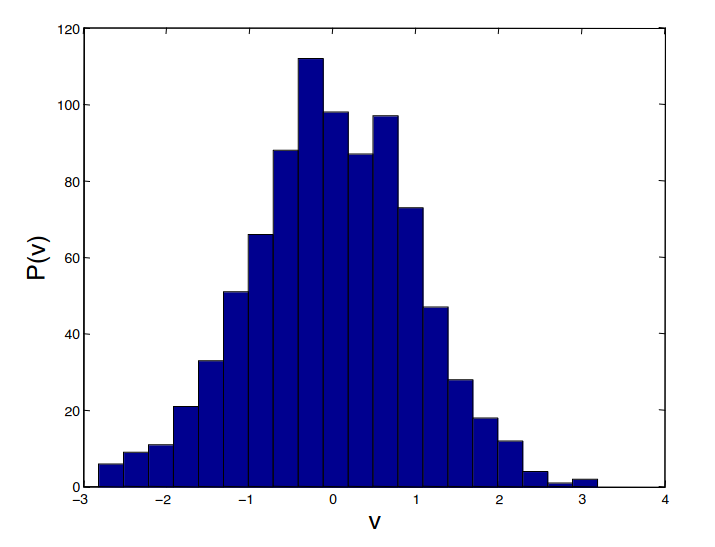
\includegraphics[width=0.5\textwidth]{./figs/MB_distribution.png}
\caption{Sampling velocities that follow a Maxwell-Boltzmann distribution.}
\end{figure}

    \hypertarget{boundary-conditions}{%
\subsubsection{Boundary conditions}\label{boundary-conditions}}

The next ingredient needed is boundary conditions. Consider a typical
calculation that uses periodic boundary conditions, which would be used
to simulate a solid or fluid. Other boundary conditions may be used in
different contexts, e.g., for one of the Bravais lattices, free surfaces
in surface structures.

In these exercises we consider bulk simulations and assume the
\emph{minimum image convention}. Implementation of the minimum image
convention is discussed in the text and in the prior problem set. We
emphasize that the minimum image convention was popular in the early
days of computer simulations when systems had limited memory and were
less powerful than today's machines. Since we use small systems here,
the minimum image approximation is appropriate. For research purposes
that often involve supercomputers, a different strategy for lattice sums
would likely be employed.

\hypertarget{implementation-of-force-and-energy-calculations}{%
\subsection{Implementation of force and energy
calculations}\label{implementation-of-force-and-energy-calculations}}

At each time step, we have a new set of atomic positions \(\vec{r}\). To
calculate the positions at the next time step requires the accelerations
of each atom, and thus the forces on that atom from the other particles
in the system. We also would like to calculate the potential energy,
kinetic energy, pressure, and other thermodynamic quantities of
interest.

We may write the potential energy as

\(U = \frac{1}{2}\sum_{i=1}^N \sum_{j=1}^N \phi_{ij}(r_{ij})\).

where terms for \(i=j\) are omitted. Equivalently, to avoid double
counting interations and to also cut the computation time in half, we
can also write the potential energy as

\(U = \sum_{i=1}^{N-1} \sum_{j=1+i} \phi_{ij}(r_{ij})\).

To be computationally efficient, we will calculate \(U\) and the force
with the same lattice sum strategy. The second form of \(U\) is more
computationally efficient than the first form. However, for forces, we
need \(\vec{f}_{ij}\) the force exerted by atom \(j\) on atom \(i\) and
the force exerted by atom \(i\) on atom \(j\),
\(\vec{f}_ij = -\vec{f}_{ji}\). We need to accumulate both terms as we
sum over the interactions, of which one method is demonstrated in the
following code where we invoke the minimum image convention and a
distance cutoff. We additionally accumulate values for computing the
pressure.

    \begin{tcolorbox}[breakable, size=fbox, boxrule=1pt, pad at break*=1mm,colback=cellbackground, colframe=cellborder]
\prompt{In}{incolor}{3}{\boxspacing}
\begin{Verbatim}[commandchars=\\\{\}]
\PY{o}{\PYZpc{}}\PY{k}{pycat} ./code\PYZus{}exercises/forces\PYZus{}LJ.py
\end{Verbatim}
\end{tcolorbox}

    
    \begin{Verbatim}[commandchars=\\\{\}]
\textcolor{ansi-green}{import} numpy \textcolor{ansi-green}{as} np

\textcolor{ansi-green}{def} forces\_LJ\textcolor{ansi-blue}{(}a\textcolor{ansi-blue}{,} n\textcolor{ansi-blue}{,} x\textcolor{ansi-blue}{,} y\textcolor{ansi-blue}{,} z\textcolor{ansi-blue}{)}\textcolor{ansi-blue}{:}
    \textcolor{ansi-blue}{"""}
\textcolor{ansi-blue}{    Simple lattice sum for force with cutoffs and }
\textcolor{ansi-blue}{    minimum image convention }

\textcolor{ansi-blue}{    We calculate force (fx, fy, fz), energy (u), and}
\textcolor{ansi-blue}{    part of the pressure (w).}

\textcolor{ansi-blue}{    """}
    fx \textcolor{ansi-blue}{=} np\textcolor{ansi-blue}{.}zeros\textcolor{ansi-blue}{(}n\textcolor{ansi-blue}{)}
    fy \textcolor{ansi-blue}{=} np\textcolor{ansi-blue}{.}zeros\textcolor{ansi-blue}{(}n\textcolor{ansi-blue}{)}
    fz \textcolor{ansi-blue}{=} np\textcolor{ansi-blue}{.}zeros\textcolor{ansi-blue}{(}n\textcolor{ansi-blue}{)}
    u \textcolor{ansi-blue}{=} \textcolor{ansi-cyan}{0}
    w \textcolor{ansi-blue}{=} \textcolor{ansi-cyan}{0}

    \textcolor{ansi-green}{for} i \textcolor{ansi-green}{in} range\textcolor{ansi-blue}{(}n \textcolor{ansi-blue}{-} \textcolor{ansi-cyan}{1}\textcolor{ansi-blue}{)}\textcolor{ansi-blue}{:}  \textcolor{ansi-red}{\# Note limits}
        ftx \textcolor{ansi-blue}{=} \textcolor{ansi-cyan}{0}
        fty \textcolor{ansi-blue}{=} \textcolor{ansi-cyan}{0}
        ftz \textcolor{ansi-blue}{=} \textcolor{ansi-cyan}{0}
        \textcolor{ansi-green}{for} j \textcolor{ansi-green}{in} range\textcolor{ansi-blue}{(}i \textcolor{ansi-blue}{+} \textcolor{ansi-cyan}{1}\textcolor{ansi-blue}{,} n\textcolor{ansi-blue}{)}\textcolor{ansi-blue}{:}  \textcolor{ansi-red}{\# Note limits}
            \textcolor{ansi-red}{\# Minimum image convention}
            dx \textcolor{ansi-blue}{=} x\textcolor{ansi-blue}{[}j\textcolor{ansi-blue}{]} \textcolor{ansi-blue}{-} x\textcolor{ansi-blue}{[}i\textcolor{ansi-blue}{]}
            dy \textcolor{ansi-blue}{=} y\textcolor{ansi-blue}{[}j\textcolor{ansi-blue}{]} \textcolor{ansi-blue}{-} y\textcolor{ansi-blue}{[}i\textcolor{ansi-blue}{]}
            dz \textcolor{ansi-blue}{=} z\textcolor{ansi-blue}{[}j\textcolor{ansi-blue}{]} \textcolor{ansi-blue}{-} z\textcolor{ansi-blue}{[}i\textcolor{ansi-blue}{]}
            dx \textcolor{ansi-blue}{-=} round\textcolor{ansi-blue}{(}dx\textcolor{ansi-blue}{)}
            dy \textcolor{ansi-blue}{-=} round\textcolor{ansi-blue}{(}dy\textcolor{ansi-blue}{)}
            dz \textcolor{ansi-blue}{-=} round\textcolor{ansi-blue}{(}dz\textcolor{ansi-blue}{)}
            dist \textcolor{ansi-blue}{=} a \textcolor{ansi-blue}{*} np\textcolor{ansi-blue}{.}sqrt\textcolor{ansi-blue}{(}dx\textcolor{ansi-blue}{**}\textcolor{ansi-cyan}{2} \textcolor{ansi-blue}{+} dy\textcolor{ansi-blue}{**}\textcolor{ansi-cyan}{2} \textcolor{ansi-blue}{+} dz\textcolor{ansi-blue}{**}\textcolor{ansi-cyan}{2}\textcolor{ansi-blue}{)}
            \textcolor{ansi-green}{if} dist \textcolor{ansi-blue}{<=} rc\textcolor{ansi-blue}{:}
                dphi \textcolor{ansi-blue}{=} \textcolor{ansi-blue}{(}\textcolor{ansi-cyan}{2} \textcolor{ansi-blue}{/} dist\textcolor{ansi-blue}{**}\textcolor{ansi-cyan}{12} \textcolor{ansi-blue}{-} \textcolor{ansi-cyan}{1} \textcolor{ansi-blue}{/} dist\textcolor{ansi-blue}{**}\textcolor{ansi-cyan}{6}\textcolor{ansi-blue}{)}
                ffx \textcolor{ansi-blue}{=} dphi \textcolor{ansi-blue}{*} a \textcolor{ansi-blue}{*} dx \textcolor{ansi-blue}{/} dist\textcolor{ansi-blue}{**}\textcolor{ansi-cyan}{2}
                ffy \textcolor{ansi-blue}{=} dphi \textcolor{ansi-blue}{*} a \textcolor{ansi-blue}{*} dy \textcolor{ansi-blue}{/} dist\textcolor{ansi-blue}{**}\textcolor{ansi-cyan}{2}
                ffz \textcolor{ansi-blue}{=} dphi \textcolor{ansi-blue}{*} a \textcolor{ansi-blue}{*} dz \textcolor{ansi-blue}{/} dist\textcolor{ansi-blue}{**}\textcolor{ansi-cyan}{2}
                ftx \textcolor{ansi-blue}{+=} ffx
                fty \textcolor{ansi-blue}{+=} ffy
                ftz \textcolor{ansi-blue}{+=} ffz
                phi \textcolor{ansi-blue}{=} \textcolor{ansi-blue}{(}\textcolor{ansi-cyan}{1} \textcolor{ansi-blue}{/} dist\textcolor{ansi-blue}{**}\textcolor{ansi-cyan}{12} \textcolor{ansi-blue}{-} \textcolor{ansi-cyan}{1} \textcolor{ansi-blue}{/} dist\textcolor{ansi-blue}{**}\textcolor{ansi-cyan}{6}\textcolor{ansi-blue}{)}
                u \textcolor{ansi-blue}{+=} phi
                w \textcolor{ansi-blue}{+=} dphi

                \textcolor{ansi-red}{\# Add -f to sum of force on j}
                fx\textcolor{ansi-blue}{[}j\textcolor{ansi-blue}{]} \textcolor{ansi-blue}{-=} ffx
                fy\textcolor{ansi-blue}{[}j\textcolor{ansi-blue}{]} \textcolor{ansi-blue}{-=} ffy
                fz\textcolor{ansi-blue}{[}j\textcolor{ansi-blue}{]} \textcolor{ansi-blue}{-=} ffz

        \textcolor{ansi-red}{\# Sum up force on i (fi)}
        fx\textcolor{ansi-blue}{[}i\textcolor{ansi-blue}{]} \textcolor{ansi-blue}{+=} ftx
        fy\textcolor{ansi-blue}{[}i\textcolor{ansi-blue}{]} \textcolor{ansi-blue}{+=} fty
        fz\textcolor{ansi-blue}{[}i\textcolor{ansi-blue}{]} \textcolor{ansi-blue}{+=} ftz

    \textcolor{ansi-red}{\# Need to multiply LJ by 4 and force and pressure by 24}
    \textcolor{ansi-red}{\# Also need to correct sign in f}
    u \textcolor{ansi-blue}{*=} \textcolor{ansi-cyan}{4}
    w \textcolor{ansi-blue}{*=} \textcolor{ansi-cyan}{24}
    fx \textcolor{ansi-blue}{*=} \textcolor{ansi-blue}{-}\textcolor{ansi-cyan}{24}
    fy \textcolor{ansi-blue}{*=} \textcolor{ansi-blue}{-}\textcolor{ansi-cyan}{24}
    fz \textcolor{ansi-blue}{*=} \textcolor{ansi-blue}{-}\textcolor{ansi-cyan}{24}

    \textcolor{ansi-green}{return} u\textcolor{ansi-blue}{,} w\textcolor{ansi-blue}{,} fx\textcolor{ansi-blue}{,} fy\textcolor{ansi-blue}{,} fz

    \end{Verbatim}

    
    Note that the data structure is somewhat different in this version of
the code In earlier codes, we defined a vector \texttt{s(i,alpha)},
which returned the components \(x\) of \texttt{s} for
\texttt{alpha\ =\ 0}, \(y\) components for \texttt{alpha\ =\ 1}, and
\(z\) components for \texttt{alpha\ =\ 2}. We use the variables
\texttt{x(j),\ y(j),\ z(j)} for each atom to make the code easier to
follow.

    \hypertarget{implementation-of-verlet-algorithm}{%
\subsection{Implementation of Verlet
algorithm}\label{implementation-of-verlet-algorithm}}

    By choice, we write all atomic positions in fractional coordinates.
Here, we show an implementation of the Verlet algorithm for the time
propagation of an MD simulation involving a \emph{cubic} simulation cell
with lattice parameter \(a\). Note where all the places \(a\) appears.

The relevant parameters are: - \texttt{nc}: number of fcc unit cells, as
described in our previous set of exercises - \texttt{density}:
volumetric density in reduced units - \texttt{tin}: input temperature in
reduced units - \texttt{nsteps}: total number of time steps in a
calculation - \texttt{dt}: time step in reduced units

The basic code is shown below.

    \begin{tcolorbox}[breakable, size=fbox, boxrule=1pt, pad at break*=1mm,colback=cellbackground, colframe=cellborder]
\prompt{In}{incolor}{4}{\boxspacing}
\begin{Verbatim}[commandchars=\\\{\}]
\PY{o}{\PYZpc{}}\PY{k}{pycat} ./code\PYZus{}exercises/MD\PYZus{}LJ.py
\end{Verbatim}
\end{tcolorbox}

    
    \begin{Verbatim}[commandchars=\\\{\}]
\textcolor{ansi-green}{import} numpy \textcolor{ansi-green}{as} np

\textcolor{ansi-green}{def} MDLJ\textcolor{ansi-blue}{(}density\textcolor{ansi-blue}{,} tin\textcolor{ansi-blue}{,} nsteps\textcolor{ansi-blue}{,} dt\textcolor{ansi-blue}{)}\textcolor{ansi-blue}{:}
    \textcolor{ansi-blue}{"""}
\textcolor{ansi-blue}{    Initialize positions and velocities.}
\textcolor{ansi-blue}{    Calculate some useful quantities.}
\textcolor{ansi-blue}{    Calculate initial energy and forces.}
\textcolor{ansi-blue}{    Now start the time stepping with the Verlet algorithm.}
\textcolor{ansi-blue}{    """}
    \textcolor{ansi-red}{\# Initialize positions and velocities}
    n\textcolor{ansi-blue}{,} x\textcolor{ansi-blue}{,} y\textcolor{ansi-blue}{,} z\textcolor{ansi-blue}{,} vx\textcolor{ansi-blue}{,} vy\textcolor{ansi-blue}{,} vz \textcolor{ansi-blue}{=} initLJMD\textcolor{ansi-blue}{(}nc\textcolor{ansi-blue}{,} tin\textcolor{ansi-blue}{)}

    \textcolor{ansi-red}{\# Calculate some useful quantities}
    vol \textcolor{ansi-blue}{=} n \textcolor{ansi-blue}{/} density
    a \textcolor{ansi-blue}{=} vol\textcolor{ansi-blue}{**}\textcolor{ansi-blue}{(}\textcolor{ansi-cyan}{1}\textcolor{ansi-blue}{/}\textcolor{ansi-cyan}{3}\textcolor{ansi-blue}{)}
    rc \textcolor{ansi-blue}{=} a \textcolor{ansi-blue}{/} \textcolor{ansi-cyan}{2}

    \textcolor{ansi-red}{\# Calculate initial energy and forces}
    u\textcolor{ansi-blue}{,} w\textcolor{ansi-blue}{,} fx\textcolor{ansi-blue}{,} fy\textcolor{ansi-blue}{,} fz \textcolor{ansi-blue}{=} forces\_LJ\textcolor{ansi-blue}{(}a\textcolor{ansi-blue}{,} n\textcolor{ansi-blue}{,} rc\textcolor{ansi-blue}{,} s\textcolor{ansi-blue}{)}

    \textcolor{ansi-red}{\# Initialize variables}
    xold \textcolor{ansi-blue}{=} np\textcolor{ansi-blue}{.}zeros\textcolor{ansi-blue}{(}n\textcolor{ansi-blue}{)}
    yold \textcolor{ansi-blue}{=} np\textcolor{ansi-blue}{.}zeros\textcolor{ansi-blue}{(}n\textcolor{ansi-blue}{)}
    zold \textcolor{ansi-blue}{=} np\textcolor{ansi-blue}{.}zeros\textcolor{ansi-blue}{(}n\textcolor{ansi-blue}{)}
    xnew \textcolor{ansi-blue}{=} np\textcolor{ansi-blue}{.}zeros\textcolor{ansi-blue}{(}n\textcolor{ansi-blue}{)}
    ynew \textcolor{ansi-blue}{=} np\textcolor{ansi-blue}{.}zeros\textcolor{ansi-blue}{(}n\textcolor{ansi-blue}{)}
    znew \textcolor{ansi-blue}{=} np\textcolor{ansi-blue}{.}zeros\textcolor{ansi-blue}{(}n\textcolor{ansi-blue}{)}
    
    \textcolor{ansi-red}{\# Time series arrays}
    un \textcolor{ansi-blue}{=} np\textcolor{ansi-blue}{.}zeros\textcolor{ansi-blue}{(}nsteps\textcolor{ansi-blue}{)}
    kn \textcolor{ansi-blue}{=} np\textcolor{ansi-blue}{.}zeros\textcolor{ansi-blue}{(}nsteps\textcolor{ansi-blue}{)}
    en \textcolor{ansi-blue}{=} np\textcolor{ansi-blue}{.}zeros\textcolor{ansi-blue}{(}nsteps\textcolor{ansi-blue}{)}
    tn \textcolor{ansi-blue}{=} np\textcolor{ansi-blue}{.}zeros\textcolor{ansi-blue}{(}nsteps\textcolor{ansi-blue}{)}
    pn \textcolor{ansi-blue}{=} np\textcolor{ansi-blue}{.}zeros\textcolor{ansi-blue}{(}nsteps\textcolor{ansi-blue}{)}

    \textcolor{ansi-red}{\# First find the positions at t-dt}
    \textcolor{ansi-green}{for} i \textcolor{ansi-green}{in} range\textcolor{ansi-blue}{(}n\textcolor{ansi-blue}{)}\textcolor{ansi-blue}{:}
        xold\textcolor{ansi-blue}{[}i\textcolor{ansi-blue}{]} \textcolor{ansi-blue}{=} x\textcolor{ansi-blue}{[}i\textcolor{ansi-blue}{]} \textcolor{ansi-blue}{-} vx\textcolor{ansi-blue}{[}i\textcolor{ansi-blue}{]}\textcolor{ansi-blue}{*}dt\textcolor{ansi-blue}{/}a \textcolor{ansi-blue}{+} \textcolor{ansi-cyan}{0.5}\textcolor{ansi-blue}{*}fx\textcolor{ansi-blue}{[}i\textcolor{ansi-blue}{]}\textcolor{ansi-blue}{*}dt\textcolor{ansi-blue}{**}\textcolor{ansi-cyan}{2}\textcolor{ansi-blue}{/}a
        yold\textcolor{ansi-blue}{[}i\textcolor{ansi-blue}{]} \textcolor{ansi-blue}{=} y\textcolor{ansi-blue}{[}i\textcolor{ansi-blue}{]} \textcolor{ansi-blue}{-} vy\textcolor{ansi-blue}{[}i\textcolor{ansi-blue}{]}\textcolor{ansi-blue}{*}dt\textcolor{ansi-blue}{/}a \textcolor{ansi-blue}{+} \textcolor{ansi-cyan}{0.5}\textcolor{ansi-blue}{*}fy\textcolor{ansi-blue}{[}i\textcolor{ansi-blue}{]}\textcolor{ansi-blue}{*}dt\textcolor{ansi-blue}{**}\textcolor{ansi-cyan}{2}\textcolor{ansi-blue}{/}a
        zold\textcolor{ansi-blue}{[}i\textcolor{ansi-blue}{]} \textcolor{ansi-blue}{=} z\textcolor{ansi-blue}{[}i\textcolor{ansi-blue}{]} \textcolor{ansi-blue}{-} vz\textcolor{ansi-blue}{[}i\textcolor{ansi-blue}{]}\textcolor{ansi-blue}{*}dt\textcolor{ansi-blue}{/}a \textcolor{ansi-blue}{+} \textcolor{ansi-cyan}{0.5}\textcolor{ansi-blue}{*}fz\textcolor{ansi-blue}{[}i\textcolor{ansi-blue}{]}\textcolor{ansi-blue}{*}dt\textcolor{ansi-blue}{**}\textcolor{ansi-cyan}{2}\textcolor{ansi-blue}{/}a

    \textcolor{ansi-red}{\# Start the time steps}
    \textcolor{ansi-green}{for} j \textcolor{ansi-green}{in} range\textcolor{ansi-blue}{(}nsteps\textcolor{ansi-blue}{)}\textcolor{ansi-blue}{:}
        k \textcolor{ansi-blue}{=} \textcolor{ansi-cyan}{0}
        \textcolor{ansi-red}{\# Find positions for time t + dt and velocities for time t}
        \textcolor{ansi-green}{for} i \textcolor{ansi-green}{in} range\textcolor{ansi-blue}{(}n\textcolor{ansi-blue}{)}\textcolor{ansi-blue}{:}
            xnew\textcolor{ansi-blue}{[}i\textcolor{ansi-blue}{]} \textcolor{ansi-blue}{=} \textcolor{ansi-cyan}{2}\textcolor{ansi-blue}{*}x\textcolor{ansi-blue}{[}i\textcolor{ansi-blue}{]} \textcolor{ansi-blue}{-} xold\textcolor{ansi-blue}{[}i\textcolor{ansi-blue}{]} \textcolor{ansi-blue}{+} fx\textcolor{ansi-blue}{[}i\textcolor{ansi-blue}{]}\textcolor{ansi-blue}{*}dt\textcolor{ansi-blue}{**}\textcolor{ansi-cyan}{2}\textcolor{ansi-blue}{/}a
            ynew\textcolor{ansi-blue}{[}i\textcolor{ansi-blue}{]} \textcolor{ansi-blue}{=} \textcolor{ansi-cyan}{2}\textcolor{ansi-blue}{*}y\textcolor{ansi-blue}{[}i\textcolor{ansi-blue}{]} \textcolor{ansi-blue}{-} yold\textcolor{ansi-blue}{[}i\textcolor{ansi-blue}{]} \textcolor{ansi-blue}{+} fy\textcolor{ansi-blue}{[}i\textcolor{ansi-blue}{]}\textcolor{ansi-blue}{*}dt\textcolor{ansi-blue}{**}\textcolor{ansi-cyan}{2}\textcolor{ansi-blue}{/}a
            znew\textcolor{ansi-blue}{[}i\textcolor{ansi-blue}{]} \textcolor{ansi-blue}{=} \textcolor{ansi-cyan}{2}\textcolor{ansi-blue}{*}z\textcolor{ansi-blue}{[}i\textcolor{ansi-blue}{]} \textcolor{ansi-blue}{-} zold\textcolor{ansi-blue}{[}i\textcolor{ansi-blue}{]} \textcolor{ansi-blue}{+} fz\textcolor{ansi-blue}{[}i\textcolor{ansi-blue}{]}\textcolor{ansi-blue}{*}dt\textcolor{ansi-blue}{**}\textcolor{ansi-cyan}{2}\textcolor{ansi-blue}{/}a
            vx\textcolor{ansi-blue}{[}i\textcolor{ansi-blue}{]} \textcolor{ansi-blue}{=} a\textcolor{ansi-blue}{*}\textcolor{ansi-blue}{(}xnew\textcolor{ansi-blue}{[}i\textcolor{ansi-blue}{]} \textcolor{ansi-blue}{-} xold\textcolor{ansi-blue}{[}i\textcolor{ansi-blue}{]}\textcolor{ansi-blue}{)} \textcolor{ansi-blue}{/} \textcolor{ansi-blue}{(}\textcolor{ansi-cyan}{2}\textcolor{ansi-blue}{*}dt\textcolor{ansi-blue}{)}
            vy\textcolor{ansi-blue}{[}i\textcolor{ansi-blue}{]} \textcolor{ansi-blue}{=} a\textcolor{ansi-blue}{*}\textcolor{ansi-blue}{(}ynew\textcolor{ansi-blue}{[}i\textcolor{ansi-blue}{]} \textcolor{ansi-blue}{-} yold\textcolor{ansi-blue}{[}i\textcolor{ansi-blue}{]}\textcolor{ansi-blue}{)} \textcolor{ansi-blue}{/} \textcolor{ansi-blue}{(}\textcolor{ansi-cyan}{2}\textcolor{ansi-blue}{*}dt\textcolor{ansi-blue}{)}
            vz\textcolor{ansi-blue}{[}i\textcolor{ansi-blue}{]} \textcolor{ansi-blue}{=} a\textcolor{ansi-blue}{*}\textcolor{ansi-blue}{(}znew\textcolor{ansi-blue}{[}i\textcolor{ansi-blue}{]} \textcolor{ansi-blue}{-} zold\textcolor{ansi-blue}{[}i\textcolor{ansi-blue}{]}\textcolor{ansi-blue}{)} \textcolor{ansi-blue}{/} \textcolor{ansi-blue}{(}\textcolor{ansi-cyan}{2}\textcolor{ansi-blue}{*}dt\textcolor{ansi-blue}{)}
            k \textcolor{ansi-blue}{+=} vx\textcolor{ansi-blue}{[}i\textcolor{ansi-blue}{]}\textcolor{ansi-blue}{**}\textcolor{ansi-cyan}{2} \textcolor{ansi-blue}{+} vy\textcolor{ansi-blue}{[}i\textcolor{ansi-blue}{]}\textcolor{ansi-blue}{**}\textcolor{ansi-cyan}{2} \textcolor{ansi-blue}{+} vz\textcolor{ansi-blue}{[}i\textcolor{ansi-blue}{]}\textcolor{ansi-blue}{**}\textcolor{ansi-cyan}{2}

        k \textcolor{ansi-blue}{*=} \textcolor{ansi-cyan}{0.5}
        temp \textcolor{ansi-blue}{=} \textcolor{ansi-cyan}{2}\textcolor{ansi-blue}{*}k \textcolor{ansi-blue}{/} \textcolor{ansi-blue}{(}\textcolor{ansi-cyan}{3}\textcolor{ansi-blue}{*}n\textcolor{ansi-blue}{)}

        \textcolor{ansi-red}{\# Create time series of values}
        e \textcolor{ansi-blue}{=} k \textcolor{ansi-blue}{+} u
        un\textcolor{ansi-blue}{[}j\textcolor{ansi-blue}{]} \textcolor{ansi-blue}{=} u \textcolor{ansi-blue}{/} n
        kn\textcolor{ansi-blue}{[}j\textcolor{ansi-blue}{]} \textcolor{ansi-blue}{=} k \textcolor{ansi-blue}{/} n
        en\textcolor{ansi-blue}{[}j\textcolor{ansi-blue}{]} \textcolor{ansi-blue}{=} e \textcolor{ansi-blue}{/} n
        tn\textcolor{ansi-blue}{[}j\textcolor{ansi-blue}{]} \textcolor{ansi-blue}{=} temp
        pn\textcolor{ansi-blue}{[}j\textcolor{ansi-blue}{]} \textcolor{ansi-blue}{=} density\textcolor{ansi-blue}{*}temp \textcolor{ansi-blue}{+} w \textcolor{ansi-blue}{/} \textcolor{ansi-blue}{(}\textcolor{ansi-cyan}{3}\textcolor{ansi-blue}{*}vol\textcolor{ansi-blue}{)}

        \textcolor{ansi-red}{\# Reset positions for next time step}
        \textcolor{ansi-green}{for} i \textcolor{ansi-green}{in} range\textcolor{ansi-blue}{(}n\textcolor{ansi-blue}{)}\textcolor{ansi-blue}{:}
            xold\textcolor{ansi-blue}{[}i\textcolor{ansi-blue}{]}\textcolor{ansi-blue}{,} yold\textcolor{ansi-blue}{[}i\textcolor{ansi-blue}{]}\textcolor{ansi-blue}{,} zold\textcolor{ansi-blue}{[}i\textcolor{ansi-blue}{]} \textcolor{ansi-blue}{=} x\textcolor{ansi-blue}{[}i\textcolor{ansi-blue}{]}\textcolor{ansi-blue}{,} y\textcolor{ansi-blue}{[}i\textcolor{ansi-blue}{]}\textcolor{ansi-blue}{,} z\textcolor{ansi-blue}{[}i\textcolor{ansi-blue}{]}
            x\textcolor{ansi-blue}{[}i\textcolor{ansi-blue}{]}\textcolor{ansi-blue}{,} y\textcolor{ansi-blue}{[}i\textcolor{ansi-blue}{]}\textcolor{ansi-blue}{,} z\textcolor{ansi-blue}{[}i\textcolor{ansi-blue}{]} \textcolor{ansi-blue}{=} xnew\textcolor{ansi-blue}{[}i\textcolor{ansi-blue}{]}\textcolor{ansi-blue}{,} ynew\textcolor{ansi-blue}{[}i\textcolor{ansi-blue}{]}\textcolor{ansi-blue}{,} znew\textcolor{ansi-blue}{[}i\textcolor{ansi-blue}{]}

        \textcolor{ansi-red}{\# Calculate force and energy at new positions for next cycle}
        u\textcolor{ansi-blue}{,} w\textcolor{ansi-blue}{,} fx\textcolor{ansi-blue}{,} fy\textcolor{ansi-blue}{,} fz \textcolor{ansi-blue}{=} forces\_LJ\textcolor{ansi-blue}{(}a\textcolor{ansi-blue}{,} n\textcolor{ansi-blue}{,} rc\textcolor{ansi-blue}{,} x\textcolor{ansi-blue}{,} y\textcolor{ansi-blue}{,} z\textcolor{ansi-blue}{)}

    \textcolor{ansi-green}{return} un\textcolor{ansi-blue}{,} kn\textcolor{ansi-blue}{,} en\textcolor{ansi-blue}{,} tn\textcolor{ansi-blue}{,} pn

    \end{Verbatim}

    
    \hypertarget{determine-if-the-md-simulation-is-properly-working}{%
\subsubsection{Determine if the MD simulation is properly
working}\label{determine-if-the-md-simulation-is-properly-working}}

With this bare bones implementation, we need to see if our MD simulation
works appropriately. Usually, one has to consider if: 1) the code is
written correctly or 2) if the user is using the code correctly. We can
answer both to a certain degree with test against physically known
principles.

Here, we use the most fundamental of physically known principles, the
conservation of total energy over time, i.e., \(E = K+U\). We will
expect some fluctuations in the energy over time (and in certain cases
these fluctuations contain important thermodynamic information).
However, the fluctuations should be relatively small and the
time-average of the total energy \(\langle E \rangle\) should remain
constant and not drift with time. A rule of thumb is

\(\frac{\text{max}(E) - \text{min}(E)}{\langle E \rangle} \sim 10^{-4}\)

where \(\text{max}(E) - \text{min}(E)\) is the range of values of \(E\).
If \(\langle E \rangle\) is small, then you must correpsondingly adjust
this criteria.

If your total energies begin drifting with time, there are a few places
to look first. 1) There is an error in code. You will need to debug the
code. 2) Your timestep \(dt\) is too large, which leads to inaccuracies
in the solution to the constitutive equations (here, Newton's equations)
that can lead to large fluctuations in E and drifiting over time. As a
rule of thumb, your \(dt\) should be small enough able to capture the
highest frequencies of vibrations to capture the physics of the system
but not too small that you are wasting computational time. 3) Your
potential has large gradients and the algorithm you have chosen to solve
the equations of motion are unstable and/or inadequate. Here we choose
the Verlet algorithm, which for toy systems performs suitably well.
However, more complex potentials or simulations require additional
considerations.

Other fundamental thermodynamic or physical relationships may also need
to be enforced in the MD simulation. At minimum, the conservation of
energy must be conserved.

It is worth noting that substantial work often goes into coding the
potential function in research-level calculations. Checking for errors
in the coding of the potential is also an important task. Such errors
may not be obvious to detect, so one often turns to established
knowledge or well-studied model systems (i.e., replicating prior
literature results from someone else's calculation or some result from
experiment).

As computational scientists, we think about - verifying the code: the
code works correctly - validating the code: the code gives a reliable
description of the physical system of interest

Beyond checking that the code works, one may think of code dissemination
along the principle of FAIR (https://www.go-fair.org/fair-principles/).
At the basic level, this consists of e.g., having readable code,
thoroughly commenting your code, and making sure each version passes a
set of pre-determined tests. In Python, there are recommended style
guides and conventions (https://peps.python.org/pep-0008/). For large
and mature codes, this often involves developing extensive user and
developer documentation, including user tutorials and hosting user
forums.

    \hypertarget{exercises}{%
\section{=============== Exercises ===============}\label{exercises}}

    We will study two types of systems: - a simple model of atoms on a
surface, starting with a single atom - a bulk system described by an
empirical potential (i.e., Lennard-Jones potential)

    \hypertarget{atoms-on-a-surface}{%
\subsubsection{Atoms on a surface}\label{atoms-on-a-surface}}

We start with a simple toy model that will help demonstrate the basics
of molecular dynamics simulations. Let's suppose we have a rigid surface
that contains some atoms (starting with one) on the surface. There is an
exchange of energy between the surface and atoms moving on top of the
surface. The interaction between the surface and atom(s) is described
with a simple potential that is not designed to represent a realistic
material. Regardless, there are several interesting states that are
possible to drive the system into that are analogous to realistic
systems.

We define our potential to be

\(\phi(x,y) = A\sin(\pi x)\cos(\pi y)\)

where \(A\) is some adjustable parameter that represents the strength of
interaction. As usual, the force is the negative of the gradient of the
potential.

We can then easily implement the potential and force.

    We still start with the simulation of a single atom. Since
``temperature'' is a thermodynamic statistical average, it will be
difficult to define an input target temperature. Instead, we will input
the total energy, \texttt{ein}. We need to somehow initialize the
surface before letting the molecular dynamics simulation to proceed.

First, we will first a random position near a well, calculate the
potential and use \(K=E-U\) to define a kinetic energy. Random
velocities will be generated and then rescaled to give the appropriate
\(K\).

    \begin{tcolorbox}[breakable, size=fbox, boxrule=1pt, pad at break*=1mm,colback=cellbackground, colframe=cellborder]
\prompt{In}{incolor}{5}{\boxspacing}
\begin{Verbatim}[commandchars=\\\{\}]
\PY{o}{\PYZpc{}}\PY{k}{pycat} ./code\PYZus{}exercises/2Dsurf.py
\end{Verbatim}
\end{tcolorbox}

    
    \begin{Verbatim}[commandchars=\\\{\}]
\textcolor{ansi-green}{import} numpy \textcolor{ansi-green}{as} np

\textcolor{ansi-red}{\# 2D surface}

\textcolor{ansi-green}{def} phisurf\textcolor{ansi-blue}{(}acon\textcolor{ansi-blue}{,} x\textcolor{ansi-blue}{,} y\textcolor{ansi-blue}{)}\textcolor{ansi-blue}{:}
    \textcolor{ansi-blue}{"""}
\textcolor{ansi-blue}{    Surface potential}
\textcolor{ansi-blue}{    """}
    phi \textcolor{ansi-blue}{=} acon \textcolor{ansi-blue}{*} np\textcolor{ansi-blue}{.}sin\textcolor{ansi-blue}{(}np\textcolor{ansi-blue}{.}pi \textcolor{ansi-blue}{*} x\textcolor{ansi-blue}{)} \textcolor{ansi-blue}{*} np\textcolor{ansi-blue}{.}sin\textcolor{ansi-blue}{(}np\textcolor{ansi-blue}{.}pi \textcolor{ansi-blue}{*} y\textcolor{ansi-blue}{)}
    \textcolor{ansi-green}{return} phi

\textcolor{ansi-green}{def} fsurf\textcolor{ansi-blue}{(}acon\textcolor{ansi-blue}{,} x\textcolor{ansi-blue}{,} y\textcolor{ansi-blue}{)}\textcolor{ansi-blue}{:}
    \textcolor{ansi-blue}{"""}
\textcolor{ansi-blue}{    Surface force}
\textcolor{ansi-blue}{    """}
    fx \textcolor{ansi-blue}{=} \textcolor{ansi-blue}{-}acon \textcolor{ansi-blue}{*} np\textcolor{ansi-blue}{.}pi \textcolor{ansi-blue}{*} np\textcolor{ansi-blue}{.}cos\textcolor{ansi-blue}{(}np\textcolor{ansi-blue}{.}pi \textcolor{ansi-blue}{*} x\textcolor{ansi-blue}{)} \textcolor{ansi-blue}{*} np\textcolor{ansi-blue}{.}sin\textcolor{ansi-blue}{(}np\textcolor{ansi-blue}{.}pi \textcolor{ansi-blue}{*} y\textcolor{ansi-blue}{)}
    fy \textcolor{ansi-blue}{=} \textcolor{ansi-blue}{-}acon \textcolor{ansi-blue}{*} np\textcolor{ansi-blue}{.}pi \textcolor{ansi-blue}{*} np\textcolor{ansi-blue}{.}sin\textcolor{ansi-blue}{(}np\textcolor{ansi-blue}{.}pi \textcolor{ansi-blue}{*} x\textcolor{ansi-blue}{)} \textcolor{ansi-blue}{*} np\textcolor{ansi-blue}{.}cos\textcolor{ansi-blue}{(}np\textcolor{ansi-blue}{.}pi \textcolor{ansi-blue}{*} y\textcolor{ansi-blue}{)}
    \textcolor{ansi-green}{return} fx\textcolor{ansi-blue}{,} fy


\textcolor{ansi-green}{def} initsurf\textcolor{ansi-blue}{(}ein\textcolor{ansi-blue}{,} acon\textcolor{ansi-blue}{)}\textcolor{ansi-blue}{:}
    \textcolor{ansi-blue}{"""}
\textcolor{ansi-blue}{    Pick x and y so they sit near a well}
\textcolor{ansi-blue}{    """}
    x \textcolor{ansi-blue}{=} \textcolor{ansi-blue}{-}\textcolor{ansi-cyan}{0.75} \textcolor{ansi-blue}{+} \textcolor{ansi-cyan}{1.5} \textcolor{ansi-blue}{*} np\textcolor{ansi-blue}{.}random\textcolor{ansi-blue}{.}rand\textcolor{ansi-blue}{(}\textcolor{ansi-blue}{)}
    y \textcolor{ansi-blue}{=} \textcolor{ansi-blue}{-}\textcolor{ansi-cyan}{0.75} \textcolor{ansi-blue}{+} \textcolor{ansi-cyan}{1.5} \textcolor{ansi-blue}{*} np\textcolor{ansi-blue}{.}random\textcolor{ansi-blue}{.}rand\textcolor{ansi-blue}{(}\textcolor{ansi-blue}{)}

    \textcolor{ansi-red}{\# Calculate potential at x, y}
    phi \textcolor{ansi-blue}{=} phisurf\textcolor{ansi-blue}{(}acon\textcolor{ansi-blue}{,} x\textcolor{ansi-blue}{,} y\textcolor{ansi-blue}{)}

    \textcolor{ansi-red}{\# Find kinetic energy such that total energy is ein}
    ki \textcolor{ansi-blue}{=} ein \textcolor{ansi-blue}{-} phi

    \textcolor{ansi-red}{\# Pick random velocity components}
    vxs \textcolor{ansi-blue}{=} np\textcolor{ansi-blue}{.}random\textcolor{ansi-blue}{.}rand\textcolor{ansi-blue}{(}\textcolor{ansi-blue}{)}
    vys \textcolor{ansi-blue}{=} np\textcolor{ansi-blue}{.}random\textcolor{ansi-blue}{.}rand\textcolor{ansi-blue}{(}\textcolor{ansi-blue}{)}

    \textcolor{ansi-red}{\# Find kinetic energy from random velocities}
    ks \textcolor{ansi-blue}{=} \textcolor{ansi-cyan}{0.5} \textcolor{ansi-blue}{*} \textcolor{ansi-blue}{(}vxs\textcolor{ansi-blue}{**}\textcolor{ansi-cyan}{2} \textcolor{ansi-blue}{+} vys\textcolor{ansi-blue}{**}\textcolor{ansi-cyan}{2}\textcolor{ansi-blue}{)}

    \textcolor{ansi-red}{\# Scale velocities so total energy is equal to ein}
    vx \textcolor{ansi-blue}{=} vxs \textcolor{ansi-blue}{*} np\textcolor{ansi-blue}{.}sqrt\textcolor{ansi-blue}{(}ki \textcolor{ansi-blue}{/} ks\textcolor{ansi-blue}{)}
    vy \textcolor{ansi-blue}{=} vys \textcolor{ansi-blue}{*} np\textcolor{ansi-blue}{.}sqrt\textcolor{ansi-blue}{(}ki \textcolor{ansi-blue}{/} ks\textcolor{ansi-blue}{)}

    \textcolor{ansi-green}{return} x\textcolor{ansi-blue}{,} y\textcolor{ansi-blue}{,} vx\textcolor{ansi-blue}{,} vy

    \end{Verbatim}

    
    We will use the Verlet algorithm to solve the equations of motion in two
dimensions. The discussion of the code involved so far is sufficient to
start testing all of the functions with our simple 2D potential model.

    \hypertarget{single-atom-on-surface}{%
\subsection{==== Single atom on surface
====}\label{single-atom-on-surface}}

    \begin{enumerate}
\def\labelenumi{\arabic{enumi}.}
\tightlist
\item
  Using the Verlet algorithm, implement an MD code to explore the ``atom
  on a surface'' problem. Do not use periodic boundary conditions so
  that you may monitor large motions of your atom(s). Use \(E\) as an
  input parameter. You may use the provided code in constructing the MD
  code or implement the routines yourself.
\end{enumerate}

\begin{enumerate}
\def\labelenumi{\alph{enumi})}
\tightlist
\item
  Vary the time step and comment on the numerical error. Show plots of
  the calculated total energy. Is the total energy being integrated
  properly?
\end{enumerate}

    \begin{enumerate}
\def\labelenumi{\alph{enumi})}
\setcounter{enumi}{1}
\tightlist
\item
  After determining the appropriate time step, run calculations with
  several values of \(E\). What is the relationships you observe among
  \(E\), \(U\), and \(K\)?
\end{enumerate}

    \begin{enumerate}
\def\labelenumi{\alph{enumi})}
\setcounter{enumi}{2}
\tightlist
\item
  Modify your code to calculate \(\langle U \rangle\) and
  \(\langle K \rangle\). What is relationship between temperature and
  \(\langle K \rangle\)?
\end{enumerate}

    \begin{enumerate}
\def\labelenumi{\alph{enumi})}
\setcounter{enumi}{3}
\tightlist
\item
  For the same calculations, examine the behavior of the atom motion as
  a function of the energy of the atom. Comment on the relationship
  between the input energy and the ability of the atom to jump out of
  the well.
\end{enumerate}

    In all cases in d), plot the trajectory of the atom relative to the
underlying potential.

You may visualize the potential as a contour plot. In python, you may
find it helpful to define a grid of \texttt{(x,y)} coordinates in the
following manner. First, define a vector \(x\) and \(y\) values

\begin{Shaded}
\begin{Highlighting}[]
\ImportTok{import}\NormalTok{ numpy }\ImportTok{as}\NormalTok{ np}
\NormalTok{x }\OperatorTok{=}\NormalTok{ np.arange(}\OperatorTok{{-}}\DecValTok{10}\NormalTok{,}\DecValTok{10}\NormalTok{,}\FloatTok{0.1}\NormalTok{)}
\NormalTok{y }\OperatorTok{=}\NormalTok{ np.arange(}\OperatorTok{{-}}\DecValTok{10}\NormalTok{,}\DecValTok{10}\NormalTok{,}\FloatTok{0.1}\NormalTok{)}
\end{Highlighting}
\end{Shaded}

Then, use the \(x\) and \(y\) vectors to define a two-dimensional grid
using the built-in \texttt{numpy} function \texttt{meshgrid}

\begin{Shaded}
\begin{Highlighting}[]
\NormalTok{xmesh, ymesh }\OperatorTok{=}\NormalTok{ np.meshgrid(x,y)}
\end{Highlighting}
\end{Shaded}

You may then easily evaluate a function \(Z\) on the grid of coordinates
generated

\begin{Shaded}
\begin{Highlighting}[]
\NormalTok{Z }\OperatorTok{=}\NormalTok{ f(xmesh,ymesh)}
\end{Highlighting}
\end{Shaded}

and use \texttt{matplotlib} built-in function \texttt{countour} plot.

    \hypertarget{multiple-atoms-on-the-surface}{%
\subsection{Multiple atoms on the
surface}\label{multiple-atoms-on-the-surface}}

\begin{enumerate}
\def\labelenumi{\arabic{enumi}.}
\setcounter{enumi}{1}
\tightlist
\item
  Modify the code to include multiple atoms on the surface and to
  include periodic boundary conditions using the minimum image
  convention. Choose a system size that includes at least 5 surface unit
  cells in each direction. Having multiple atoms on the surface means
  interaction between the atoms is possible. We may choose to model that
  interaction with the Lennard-Jones potential (or any other appropriate
  potential).
\end{enumerate}

We showed above how to compute energy and forces with the Lennard-Jones
potential. In the above implementation, it is assumed that the periodic
surface is a square lattice with lattice parameter 1. However, the
Lennard-Jones potential in distance reduced units has its energetic
minimum at \(r_m = 2^{1/6} \approx 1.12\), which means that there would
be a 12\% mismatch between the assumed periodic surface and the
interaction potential. We can vary this mismatch with a simple
modification of the surface potential

\(\phi(x,y) = A\sin(\pi x/a)\cos(\pi y/a)\)

where \(a\) is the lattice parameter of the surface atoms, which can be
varied.

    \begin{enumerate}
\def\labelenumi{\alph{enumi})}
\tightlist
\item
  Switch from an energy-based input to a temperature-based input for the
  initial velocities. Choose the initial velocities from either a normal
  distribution or pick a set of velocity components over a small range
  centered on zero and scale to the initial temperature chosen. Choose
  initial atomic positions near minimum(s) of the surface potential.
\end{enumerate}

    \begin{enumerate}
\def\labelenumi{\alph{enumi})}
\setcounter{enumi}{1}
\tightlist
\item
  Pick two temperatures and two values for the interaction strength
  \(A\). Run calculations until you observe equilibration in the
  energies and then compare the structure of the atoms on the surface.
  Do you observe clustering, repulsion, or something else? Note to take
  the minimum-image approach to scale back atom positions that fall
  outside of the central cell.
\end{enumerate}

\begin{center}\rule{0.5\linewidth}{0.5pt}\end{center}

    \begin{enumerate}
\def\labelenumi{\arabic{enumi}.}
\setcounter{enumi}{2}
\tightlist
\item
  Repeat part 2b) with a different density of atoms on the surface.
\end{enumerate}

\begin{center}\rule{0.5\linewidth}{0.5pt}\end{center}

    \hypertarget{bulk-material}{%
\subsection{Bulk Material}\label{bulk-material}}

    The hypothetical material ``Lennard-Jonesium'' is well studied (of
course only by computation). A ``phase diagram'' of this material is
presented in the figure below.

\begin{figure}
\centering
\caption{Phase diagram of Lennard-Jonesiusm. From J. P. Hansen and L. Verlet,
``Phase transitions of the Lennard-Jones system,'' Phys.Rev. 184,
151--161 (1969).}
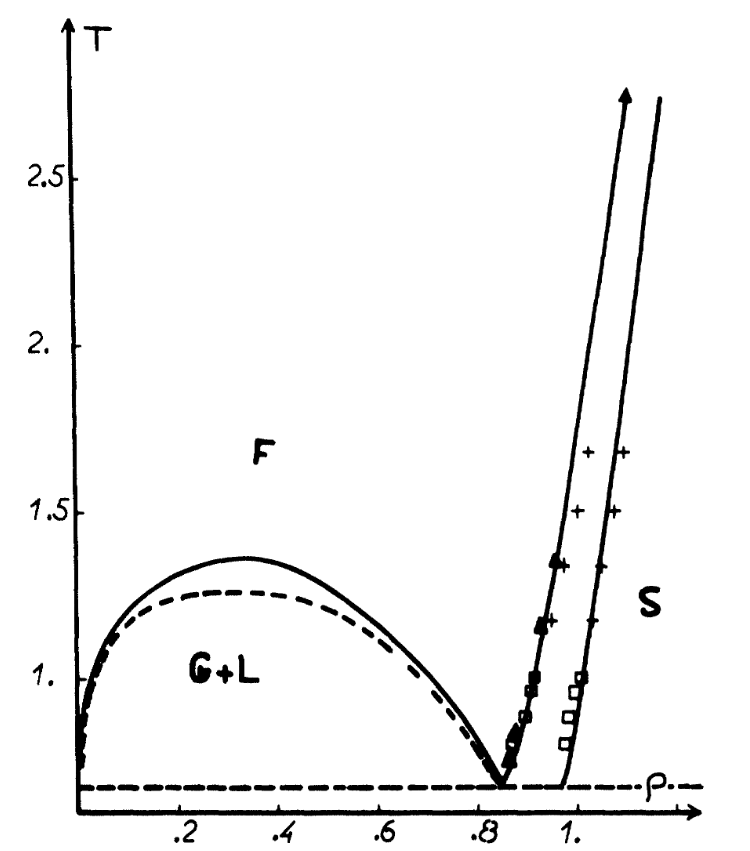
\includegraphics[width=0.5\textwidth]{./figs/LJ-phase.png}
\end{figure}

For the following exercises, you will want to restrict the densities
(\(\rho\)) and temperatures (\(T\)) to remain in the solid (S) or liquid
(L) regions. For example, at \(\rho=0\), the melting point occurs at
\(T=0.7\).

\begin{center}\rule{0.5\linewidth}{0.5pt}\end{center}

\begin{enumerate}
\def\labelenumi{\arabic{enumi}.}
\setcounter{enumi}{3}
\tightlist
\item
  Our first order of business is to determine a time step, which can
  often be estimated from what we know of the system being studied.
  Assume reduced units.
\end{enumerate}

\begin{enumerate}
\def\labelenumi{\alph{enumi})}
\item
  Estimate the approximate time step for the simulation in reduced units
  assuming a time step of \(5\times 10^{-15}\) s. Use the mass of one of
  the rare gas atoms and the appropriate potential parameters as given
  in the text.
\item
  The period of an atom in a harmonic oscillator is \(2\pi/\omega\),
  where \(\omega = \sqrt{k/m}\). For a Lennard-Jones system at zero
  pressure and temperature, one can show that the force constant
  \(k=377\varepsilon/\sigma^2\). Assuming 50 time steps per period,
  calculate the time step in reduced units and compare with (a).
\end{enumerate}

\begin{center}\rule{0.5\linewidth}{0.5pt}\end{center}

    \begin{enumerate}
\def\labelenumi{\arabic{enumi}.}
\setcounter{enumi}{4}
\tightlist
\item
  Assume some density and initial temperature for a Lennard-Jones
  system. Use a small system (i.e., \(2\times 2\times 2\) supercell of
  fcc cells (N = 32) or \(3 \times 3 \times 3\) supercell (N=108).
  Assume the time step in Problem 4. Run the system for a few hundred
  steps. Is this time step small enough, based on the energy criterion
  above? Your goal is the biggest time step possible that still gives a
  good solution. Note that for small systems it may be difficult to
  reach energy fluctuations \(< 10^{-4}\).
\end{enumerate}

\begin{center}\rule{0.5\linewidth}{0.5pt}\end{center}

    \begin{enumerate}
\def\labelenumi{\arabic{enumi}.}
\setcounter{enumi}{5}
\tightlist
\item
  Pick a density and temperature such that the material is in the
  \textbf{solid} phase. Using the selected time step, run a simulation
  long enough to reach equilibration (typically a few thousand time
  steps).
\end{enumerate}

\begin{enumerate}
\def\labelenumi{\alph{enumi})}
\item
  Plot the various thermodynamic quantities (\(E, T, K, P\)). By what
  time step has the system reached equilibrium?
\item
  Average the various thermodynamic quantities over the equilibrated
  run. Note, it may be easier to output the calculated quantities as
  time sequences and then average everything in a separate routine.
  Remember to omit the initial part of the time sequence when the system
  has not quite equilibrated.
\end{enumerate}

\begin{center}\rule{0.5\linewidth}{0.5pt}\end{center}

    \begin{enumerate}
\def\labelenumi{\arabic{enumi}.}
\setcounter{enumi}{6}
\tightlist
\item
  You may have noticed that the equilibrilation time can take awhile.
  The code in its current form takes a while to equilibrate. Currently,
  the code is written such that it \emph{always} starts from a perfect
  lattice and a set initial temperature. Thus the system must
  equilibrate each time it is run, which is rather inconvenient.
  Instead, one can run the initialization routines that sets initial
  positions and velocities first. Then you can change the input and
  outputs of the main MD routine as folows
\end{enumerate}

\begin{Shaded}
\begin{Highlighting}[]
\KeywordTok{def}\NormalTok{ MDLJi(density, nsteps, dt, natoms, x, y, z, vx, vy, vz)}
    \CommentTok{"""}
\CommentTok{    MD code for LJ atoms with initialization modification}
\CommentTok{    }
\CommentTok{    Input:}
\CommentTok{        density (float): density of Lennard{-}Jonesium}
\CommentTok{        nsteps (integer): number of time steps in MD run}
\CommentTok{        dt (float): time step}
\CommentTok{        natoms (integer): number of atoms in cell}
\CommentTok{        x, y, z (array of floats): atomic positions}
\CommentTok{        vx, vy, vz (array of floats): atomic velocities}
\CommentTok{    Output:}
\CommentTok{        un (array of floats): time series of potential energy per atom}
\CommentTok{        kn (array of floats): time series of kinetic energy per atom}
\CommentTok{        en (array of floats): time series of total energy per atom}
\CommentTok{        tn (array of floats): time series of temperature}
\CommentTok{        pn (array of floats): time series of pressure}
\CommentTok{        a (float): cell dimension}
\CommentTok{        x, y, z (array of floats): time series of atomic positions}
\CommentTok{        vx, vy, vz (array of floats): time series of atomic velocities}
\CommentTok{        }
\CommentTok{    """}
    \ControlFlowTok{return}\NormalTok{ un, kn, en, tn, pn, a, x, y, z, vx, vy, vz}
\end{Highlighting}
\end{Shaded}

then remove the call to \texttt{initLJMD} in the MD code. As the inputs
have changed from before, you may find that renaming the function may be
of help to distinguish it from previous versions.

Now the MD code reads in the positions and velocities, follows through
the calculation and outputs the \emph{final} positions and velocities.

When running the code, the MD could look like

\begin{Shaded}
\begin{Highlighting}[]
\CommentTok{\# nc (integer) = number of repeated cells}
\CommentTok{\# tin (float) = desired temperature for velocities }
\NormalTok{natoms, x, y, z, vx, vy, vz }\OperatorTok{=}\NormalTok{ initLJMD(nc, tin)}
\NormalTok{un,kn,en,tn,pn,a,x,y,z,vx,vy,vz }\OperatorTok{=}\NormalTok{ MDLJi(density, nsteps, dt, natoms, x, y, z, vx, vy, vz)}
\end{Highlighting}
\end{Shaded}

After an MD calculation, we can take \texttt{x,y,z,vx,vy,vz} (i.e., the
final positions and velocities) and restart a new MD calculation without
the need for equilibrating by calling our MD routine again

\begin{Shaded}
\begin{Highlighting}[]
\NormalTok{un,kn,en,tn,pn,a,x,y,z,vx,vy,vz }\OperatorTok{=}\NormalTok{ MDLJi(density, nsteps, dt, natoms, x, y, z, vx, vy, vz)}
\end{Highlighting}
\end{Shaded}

Modify the code accordintly and redo the calculations from Problem 4,
restarting the calculation until you have a stable and equilibrated
system. Compute averages. Analyze whether there is a drfit in the
calculation as discussed in lecture. Have you made a long enough run
(i.e., have you used enough time steps) to get good statistical
averages?

\begin{center}\rule{0.5\linewidth}{0.5pt}\end{center}

    \begin{enumerate}
\def\labelenumi{\arabic{enumi}.}
\setcounter{enumi}{7}
\tightlist
\item
  Pick a density and temperature that woud put the system in the
  \textbf{liquid} phase.
\end{enumerate}

\begin{enumerate}
\def\labelenumi{\alph{enumi})}
\item
  Using the optical time step, run a few thousand time steps (this
  should take a few minutes) and plot the various thermodynamic
  quantities.
\item
  By what time stpe has the system equilibrated?
\item
  Find average quantities over the equilibrated part of the run. Analyze
  whether there is a drift in the calculation as discussed in lecture.
  Have you have a long enough run (i.e., have you used enough time steps
  to get good statistics?
\end{enumerate}

\begin{center}\rule{0.5\linewidth}{0.5pt}\end{center}

    \begin{enumerate}
\def\labelenumi{\arabic{enumi}.}
\setcounter{enumi}{8}
\tightlist
\item
  Using the data you have generated in part 6., calculate the
  fluctuations for the various thermodynamic quantities (e.g.,
  \(\langle U \rangle^2 - \langle U^2 \rangle\)). Note: these
  fluctuations are not an estimate of the error of the calculation, but
  rather to related to other thermodynamic quantities. To estimate
  error, we need to follow the procedure of binning the data and finding
  the standard deviation of the averages in the bins. You may find it
  useful to create separate, reusable routines for evaluating statistics
  of trajectories.
\end{enumerate}

\begin{center}\rule{0.5\linewidth}{0.5pt}\end{center}

    \begin{enumerate}
\def\labelenumi{\arabic{enumi}.}
\setcounter{enumi}{9}
\tightlist
\item
  Compare your calculations for the solid and liquid phases. In order to
  determine whether you are in the solid or liquid phase, you need to
  monitor the structure of the material. For this, we turn to the radial
  distribution function \(g(r)\). The radial distribution function gives
  the probability that an atom is located within a thin shell \(r + dr\)
  away from a reference atom. It is customary to normalize the integral
  of \(g(r)\) to give the number of atoms within that distance. The
  appendix to Ch. 6 of Lesar discusses how to calculate \(g(r)\).
\end{enumerate}

Below we present a simple code to compute \(g(r)\), using the
normalization given in the text appendix. Such a code could be used as a
post-processing step once a set of atomic positions is known.

    \begin{tcolorbox}[breakable, size=fbox, boxrule=1pt, pad at break*=1mm,colback=cellbackground, colframe=cellborder]
\prompt{In}{incolor}{ }{\boxspacing}
\begin{Verbatim}[commandchars=\\\{\}]
\PY{k+kn}{import} \PY{n+nn}{numpy} \PY{k}{as} \PY{n+nn}{np}

\PY{k}{def} \PY{n+nf}{gr}\PY{p}{(}\PY{n}{a}\PY{p}{,} \PY{n}{n}\PY{p}{,} \PY{n}{x}\PY{p}{,} \PY{n}{y}\PY{p}{,} \PY{n}{z}\PY{p}{,} \PY{n}{nbin}\PY{p}{)}\PY{p}{:}
    \PY{l+s+sd}{\PYZdq{}\PYZdq{}\PYZdq{}}
\PY{l+s+sd}{    Calculate radial distribution function.}

\PY{l+s+sd}{    Input:}
\PY{l+s+sd}{        a (float): simulation cell dimension}
\PY{l+s+sd}{        n (integer): number of atoms}
\PY{l+s+sd}{        x, y, z (array of floats): atomic positions}
\PY{l+s+sd}{        nbin (integer): number of bins}
\PY{l+s+sd}{    Output:}
\PY{l+s+sd}{        bp (array): binning used in g(r)}
\PY{l+s+sd}{        ng (array): frequencies corresponding to g(r)}
\PY{l+s+sd}{    \PYZdq{}\PYZdq{}\PYZdq{}}
    \PY{c+c1}{\PYZsh{} cutoff, bin size}
    \PY{n}{rc} \PY{o}{=} \PY{n}{a} \PY{o}{/} \PY{l+m+mi}{2}
    \PY{n}{xb} \PY{o}{=} \PY{n}{rc} \PY{o}{/} \PY{n}{nbin}
    \PY{n}{g} \PY{o}{=} \PY{n}{np}\PY{o}{.}\PY{n}{zeros}\PY{p}{(}\PY{n}{nbin}\PY{p}{)}
    \PY{n}{bp} \PY{o}{=} \PY{n}{np}\PY{o}{.}\PY{n}{zeros}\PY{p}{(}\PY{n}{nbin}\PY{p}{)}
    \PY{n}{ng} \PY{o}{=} \PY{n}{np}\PY{o}{.}\PY{n}{zeros}\PY{p}{(}\PY{n}{nbin}\PY{p}{)}

    \PY{k}{for} \PY{n}{i} \PY{o+ow}{in} \PY{n+nb}{range}\PY{p}{(}\PY{n}{n} \PY{o}{\PYZhy{}} \PY{l+m+mi}{1}\PY{p}{)}\PY{p}{:}  \PY{c+c1}{\PYZsh{} Note limits }
        \PY{k}{for} \PY{n}{j} \PY{o+ow}{in} \PY{n+nb}{range}\PY{p}{(}\PY{n}{i} \PY{o}{+} \PY{l+m+mi}{1}\PY{p}{,} \PY{n}{n}\PY{p}{)}\PY{p}{:}  \PY{c+c1}{\PYZsh{} Note limits}
            \PY{c+c1}{\PYZsh{} Minimum image convention}
            \PY{n}{dx} \PY{o}{=} \PY{n}{x}\PY{p}{[}\PY{n}{j}\PY{p}{]} \PY{o}{\PYZhy{}} \PY{n}{x}\PY{p}{[}\PY{n}{i}\PY{p}{]}
            \PY{n}{dy} \PY{o}{=} \PY{n}{y}\PY{p}{[}\PY{n}{j}\PY{p}{]} \PY{o}{\PYZhy{}} \PY{n}{y}\PY{p}{[}\PY{n}{i}\PY{p}{]}
            \PY{n}{dz} \PY{o}{=} \PY{n}{z}\PY{p}{[}\PY{n}{j}\PY{p}{]} \PY{o}{\PYZhy{}} \PY{n}{z}\PY{p}{[}\PY{n}{i}\PY{p}{]}
            \PY{n}{dx} \PY{o}{\PYZhy{}}\PY{o}{=} \PY{n+nb}{round}\PY{p}{(}\PY{n}{dx}\PY{p}{)}
            \PY{n}{dy} \PY{o}{\PYZhy{}}\PY{o}{=} \PY{n+nb}{round}\PY{p}{(}\PY{n}{dy}\PY{p}{)}
            \PY{n}{dz} \PY{o}{\PYZhy{}}\PY{o}{=} \PY{n+nb}{round}\PY{p}{(}\PY{n}{dz}\PY{p}{)}
            \PY{n}{dist} \PY{o}{=} \PY{n}{a} \PY{o}{*} \PY{n}{np}\PY{o}{.}\PY{n}{sqrt}\PY{p}{(}\PY{n}{dx}\PY{o}{*}\PY{o}{*}\PY{l+m+mi}{2} \PY{o}{+} \PY{n}{dy}\PY{o}{*}\PY{o}{*}\PY{l+m+mi}{2} \PY{o}{+} \PY{n}{dz}\PY{o}{*}\PY{o}{*}\PY{l+m+mi}{2}\PY{p}{)}
            \PY{k}{if} \PY{n}{dist} \PY{o}{\PYZlt{}}\PY{o}{=} \PY{n}{rc}\PY{p}{:}
                \PY{n}{ib} \PY{o}{=} \PY{n+nb}{int}\PY{p}{(}\PY{n}{dist} \PY{o}{/} \PY{n}{xb}\PY{p}{)}
                \PY{k}{if} \PY{n}{ib} \PY{o}{\PYZlt{}} \PY{n}{nbin}\PY{p}{:}
                    \PY{n}{g}\PY{p}{[}\PY{n}{ib}\PY{p}{]} \PY{o}{+}\PY{o}{=} \PY{l+m+mi}{1}
                    
    \PY{c+c1}{\PYZsh{} For computing g(r)}
    \PY{c+c1}{\PYZsh{} Normalize and create proper distances}
    \PY{n}{factor} \PY{o}{=} \PY{l+m+mi}{2} \PY{o}{*} \PY{n}{a}\PY{o}{*}\PY{o}{*}\PY{l+m+mi}{3} \PY{o}{/} \PY{p}{(}\PY{l+m+mi}{4} \PY{o}{*} \PY{n}{np}\PY{o}{.}\PY{n}{pi} \PY{o}{*} \PY{n}{n}\PY{o}{*}\PY{o}{*}\PY{l+m+mi}{2} \PY{o}{*} \PY{n}{xb}\PY{p}{)}
    \PY{k}{for} \PY{n}{i} \PY{o+ow}{in} \PY{n+nb}{range}\PY{p}{(}\PY{n}{nbin}\PY{p}{)}\PY{p}{:}
        \PY{n}{bp}\PY{p}{[}\PY{n}{i}\PY{p}{]} \PY{o}{=} \PY{p}{(}\PY{n}{i} \PY{o}{+} \PY{l+m+mf}{0.5}\PY{p}{)} \PY{o}{*} \PY{n}{xb}
        \PY{n}{ng}\PY{p}{[}\PY{n}{i}\PY{p}{]} \PY{o}{=} \PY{n}{factor} \PY{o}{*} \PY{n}{g}\PY{p}{[}\PY{n}{i}\PY{p}{]} \PY{o}{/} \PY{p}{(}\PY{p}{(}\PY{n}{i} \PY{o}{*} \PY{n}{xb}\PY{p}{)}\PY{o}{*}\PY{o}{*}\PY{l+m+mi}{2}\PY{p}{)} \PY{k}{if} \PY{n}{i} \PY{o}{!=} \PY{l+m+mi}{0} \PY{k}{else} \PY{l+m+mi}{0}

    \PY{k}{return} \PY{n}{bp}\PY{p}{,} \PY{n}{ng}
\end{Verbatim}
\end{tcolorbox}

    From the final configuration of Problems 8 and 6, calculate \(g(r)\) for
the solid and liquid phases. For example, a command could look like

\begin{Shaded}
\begin{Highlighting}[]
\NormalTok{r,g }\OperatorTok{=}\NormalTok{ gr(a, n, x, y, z, nbin)}
\NormalTok{plt.plot(r,g)}
\end{Highlighting}
\end{Shaded}

Can you tell the difference between the structures of the solid and
liquid phases?

One of the uncertainties that you will face is that the data is noisy
when you use only the final configuration. In reality, \(g(r)\) should
be averaged over a long (equilibrated) time sequence, as it is also an
average quantity. One way to do this would be to modify the force
routine (where you already compute distances; you may have noticed the
code is similar to the force routines) and then do the binning
operations as shown in the above code. Accumulate those values and then
average at the end of the run, apply the normalization factor, and plot.
Try this.

\begin{center}\rule{0.5\linewidth}{0.5pt}\end{center}

    \begin{enumerate}
\def\labelenumi{\arabic{enumi}.}
\setcounter{enumi}{10}
\tightlist
\item
  As discussed in class, we may also define a structural order parameter
  that can discriminate between solids and liquids
\end{enumerate}

\(\rho(\vec{k}) = \frac{1}{N}\sum_{i=1}^N \cos(\vec{k}\cdot\vec{r})\).

For an fcc lattice, one may choose \(\vec{k} = (2\pi/a_{fcc})(-1,1,-1)\)
where \(a_{fcc}\) is the lattice parameter of the unit cell (not the
simulation cell). Implement a routine that computes this structural
order parameter for a final configuration of a run. Does your computed
structural order parameter agree with whether the cell is in a solid or
liquid state? How does the information from the structure order
parameter compare with \(g(r)\)?

\begin{center}\rule{0.5\linewidth}{0.5pt}\end{center}

    \begin{enumerate}
\def\labelenumi{\arabic{enumi}.}
\setcounter{enumi}{11}
\tightlist
\item
  Next, we turn to the \emph{velocity autocorrelation function}, one of
  the the most important quantities one can compute in an MD
  calculation. The velocity autocorrelation function is defined as
\end{enumerate}

\(c_{vv}(t) = \frac{m}{3k_B T}\langle \vec{v}(t) \cdot \vec{v}(0) \rangle\)

where the average \(\langle \rangle\) is taken over all particles. One
reason the velocity autocorrelation function is important is that it is
related to the diffusion constant. Compute the diffusion constant of the
fcc lattice for the solid and the liquid. What differences do you see in
the diffusion constant of the solid versus the liquid?

Hint: you will need to make the following modifications to the code.
Store the initial velocities \(v_{x0}, v_{y0}, v_{z0}\). At each time
step \(k\) calculate

\begin{Shaded}
\begin{Highlighting}[]
\NormalTok{cvv[k] }\OperatorTok{=} \DecValTok{0}

\ControlFlowTok{for}\NormalTok{ i }\KeywordTok{in}\NormalTok{ np.}\BuiltInTok{range}\NormalTok{(natoms):}
\NormalTok{    cvv[k] }\OperatorTok{=}\NormalTok{ cvv[k] }\OperatorTok{+}\NormalTok{ vxo[i]}\OperatorTok{*}\NormalTok{vx[i] }\OperatorTok{+}\NormalTok{ vyo[i]}\OperatorTok{*}\NormalTok{vy[i] }\OperatorTok{+}\NormalTok{ vzo[i]}\OperatorTok{*}\NormalTok{vz[i]}

\NormalTok{cvv[k] }\OperatorTok{=}\NormalTok{ cvv[k]}\OperatorTok{/}\NormalTok{natoms}
\end{Highlighting}
\end{Shaded}

where \(i\) the index of the index over atoms. Note that this is a very
rudimentary wayto calculate the autocorelation function. Other
approaches are discussed in the text/lecture.

\begin{center}\rule{0.5\linewidth}{0.5pt}\end{center}

    \emph{References}

\begin{enumerate}
\def\labelenumi{\arabic{enumi}.}
\item
  J.P. Hansen and L. Verlet, ``Phase transitions of the Lennard-Jones
  system.'' Phys. Rev.~184, 151-161 (1969)
\item
  R. LeSar and J.M. Rickman, ``Finite-temperature properties of
  materials from analytical statistical mechanics.'' Philosophical
  Magazine B 73, 627-639 (1996).
\end{enumerate}


    % Add a bibliography block to the postdoc
    
    
    
\end{document}
